% 正文、数字与已冻结Q1结果一致；本文件可独立编辑。
% 模板来源：https://github.com/latexstudio/CUMCMThesis，class原件保留。
% 编译：xelatex main.tex（两遍）；也可用Tectonic。
\PassOptionsToPackage{fontset=none}{ctex}
\documentclass[withoutpreface]{cumcmthesis}
% Songti/PingFang用于本机编译；其他系统自动使用发行版Fandol。
\IfFontExistsTF{Songti SC}{
  \setCJKmainfont{Songti SC}[BoldFont=Songti SC Bold]
  \setCJKsansfont{Heiti SC}
  \setCJKmonofont{Songti SC}
  \setCJKfamilyfont{zhsong}{Songti SC}
  \setCJKfamilyfont{zhhei}{Heiti SC}
  \setCJKfamilyfont{zhkai}{Songti SC}
  \setCJKfamilyfont{zhfs}{Songti SC}
}{
  \setCJKmainfont{FandolSong-Regular.otf}[BoldFont=FandolSong-Bold.otf]
  \setCJKsansfont{FandolHei-Regular.otf}[BoldFont=FandolHei-Bold.otf]
  \setCJKmonofont{FandolSong-Regular.otf}
  \setCJKfamilyfont{zhsong}{FandolSong-Regular.otf}
  \setCJKfamilyfont{zhhei}{FandolHei-Regular.otf}
  \setCJKfamilyfont{zhkai}{FandolKai-Regular.otf}
  \setCJKfamilyfont{zhfs}{FandolFang-Regular.otf}
}
\providecommand{\songti}{\CJKfamily{zhsong}}
\providecommand{\heiti}{\CJKfamily{zhhei}}
\providecommand{\kaishu}{\CJKfamily{zhkai}}
\providecommand{\fangsong}{\CJKfamily{zhfs}}
\usepackage{needspace}
\usepackage{fvextra}
\usepackage{placeins}
\usepackage{microtype}
\DeclareMathSizes{9.5}{9.5}{8}{8}
\newcommand{\important}[1]{{\heiti\bfseries #1}}
\newcommand{\questionlabel}[1]{{\heiti\bfseries\fontsize{14}{18}\selectfont #1}}
\newcommand{\topic}[1]{{\heiti\bfseries\fontsize{11}{14}\selectfont #1}}
\newcommand{\questionline}[1]{\par\noindent\hspace*{2em}{\heiti\bfseries\fontsize{14}{18}\selectfont #1\par}}
\setmainfont{texgyretermes-regular.otf}[BoldFont=texgyretermes-bold.otf,ItalicFont=texgyretermes-italic.otf,BoldItalicFont=texgyretermes-bolditalic.otf]
\setsansfont{texgyreheros-regular.otf}[BoldFont=texgyreheros-bold.otf,ItalicFont=texgyreheros-italic.otf,BoldItalicFont=texgyreheros-bolditalic.otf]
\IfFontExistsTF{Menlo}{\setmonofont{Menlo}}{\setmonofont{lmmono10-regular.otf}}
\xeCJKDeclareCharClass{CJK}{"22A5}
\geometry{a4paper,margin=25mm}
\renewcommand{\baselinestretch}{1.28}
\renewcommand{\thesection}{\chinese{section}、}
\renewcommand{\thesubsection}{\arabic{section}.\arabic{subsection}}
\renewcommand{\thefigure}{1-\arabic{figure}}
\renewcommand{\thetable}{1-\arabic{table}}
\makeatletter
\renewcommand{\mcm@cap@keywordsname}{关键词}
\renewcommand\keywords[1]{%
  \renewcommand{\mcm@tokens@keywords}{#1}%
  \par\vskip1ex
  {\noindent\zihao{-4}\heiti\bfseries\mcm@cap@keywordsname：}~{\mcm@tokens@keywords}%
}
\renewcommand\section{\@startsection{section}{1}{\z@}%
 {-3.0ex \@plus -1ex \@minus -.2ex}{1.8ex \@plus .2ex}%
 {\centering\normalfont\heiti\fontsize{14}{18}\selectfont\bfseries}}
\renewcommand\subsection{\@startsection{subsection}{2}{\z@}%
 {-1.4ex \@plus -.5ex \@minus -.2ex}{.5ex \@plus .1ex}%
 {\normalfont\heiti\fontsize{14}{18}\selectfont\bfseries}}
\renewcommand\subsubsection{\@startsection{subsubsection}{3}{2em}%
 {-1.5ex \@plus -.5ex \@minus -.2ex}{.7ex \@plus .2ex}%
 {\normalfont\heiti\fontsize{11}{14}\selectfont\bfseries}}
\makeatother
\captionsetup[figure]{font={small,normalfont},labelfont={bf},textfont={normalfont},skip=5pt}
\captionsetup[table]{font={small,normalfont},labelfont={bf},textfont={normalfont},skip=5pt}
\widowpenalty=10000 \clubpenalty=10000 \displaywidowpenalty=10000
\makeatletter
\setlength{\@fptop}{0pt}\setlength{\@fpsep}{14pt}\setlength{\@fpbot}{0pt plus 1fil}
\makeatother
\setlength{\textfloatsep}{12pt plus 3pt minus 2pt}
\setlength{\intextsep}{12pt plus 3pt minus 2pt}
\setlength{\emergencystretch}{2em}
\pagestyle{plain}
\hypersetup{pdftitle={吉隆灾害链的环境特征、触发条件、预警与仿真},pdfauthor={},pdfsubject={吉隆灾害链问题一至问题四合稿},pdfkeywords={泥石流灾害链,多尺度异常分析,剪胀—孔压耦合,触发时间预测与条件预警,多保真高斯过程,二维浅流仿真},hidelinks,pageanchor=true}
\title{吉隆灾害链的环境特征、触发条件、预警与仿真}
\date{}
\begin{document}
\pagenumbering{roman}
\pagestyle{empty}
\noindent{\heiti\fontsize{10}{12}\selectfont 队伍编号：MCB2601474\hfill 赛道：B}\par
\begin{center}
{\songti\bfseries\fontsize{16}{21}\selectfont
\begin{tabular}{@{}l@{\quad}l@{}}
题\quad 目 & \underline{吉隆灾害链的环境特征、触发条件、预警与仿真}
\end{tabular}}
\end{center}
\begin{center}
{\heiti\bfseries\fontsize{14}{18}\selectfont 摘\quad 要：}
\end{center}

2026年8月26日吉隆口岸受冰崩—碎屑流—泥石流—山洪链式灾害冲击。本文结合环境观测、事件运动与地形资料，依次研究灾前环境异常、局部起始条件、首达时间及规定入口后的传播。

\questionlabel{针对问题一，}结合站点逐小时观测与ERA5格点总降水，建立\important{年度等权多尺度历史校准}：在1、3、7、15和30日窗口构造特征，以历史参考—校准配置比较最大异常，并用主成分分析检验联合结构。从17项候选中识别格点累计总降水、2 m相对湿度、20 m减2 m气温差、10 m标量风速和格点最大小时总降水量，校准位置依次为0.902、0.869、0.854、0.852和0.845；五项在逐年剔除历史年的五次比较中均保留。30日累计降水偏高，末24—72 h偏低。

\questionlabel{针对问题二，}将湿细粒物与孔隙水理想化为饱和材料柱，依据固体守恒、水量平衡与剪胀关系建立\important{剪胀—排水—孔压耦合动力系统}，以平均有效法向应力刻画孔压反馈。二次压力剖面给出支承层起始判据：平均有效法向应力降至浮重尺度的1/6；在73 s速度窗内反求初始应力比0.17、0.30、0.50和0.75的临界累计剪切，依次为0.0188、0.520、0.981和1.35，并分析排水及压力剖面影响。

\questionlabel{针对问题三，}基于问题二的局部边界，构建\important{触发时间预测与条件预警}模型，以多分布稳健预测集合同时表达窗内首达时间与未达类别。初始应力比0.50时，相对选定计算窗起点，强施剪稳健95\%预测区间为[0.775, 0.815] s；近临界稳健95\%预测集合由有限区间[71.40, 72.95] s与窗内未达类别组成；三种速度偏移分布的模拟检验中，两条件最低单侧下界分别为0.970003和0.956011。近临界下假设发布延迟1 s、行动历时15 s，有限局部余量为[55.40, 56.95] s。

\questionlabel{针对问题四，}以规定的已形成流入口为相对时间零点，建立\important{二维守恒浅流传播模型}，并以成本感知多保真高斯过程主动学习研究局部到达边界。基准情景中局部断面约731.8 s首次达到0.1 m；四个完整河段情景的口岸断面在3600 s内未达，窗末保持运动。14次高层模拟在两条体积切片上得到摩擦系数括区[0.06000, 0.06375]和[0.07875, 0.08250]；采用\important{代理预估与物理核验}后发布到达状态。


\keywords{\important{泥石流灾害链；多尺度异常分析；剪胀—孔压耦合；触发时间预测与条件预警；多保真高斯过程；二维浅流仿真}}
\clearpage
\setcounter{tocdepth}{2}
\setlength{\cftsecnumwidth}{3em}
\tableofcontents
\thispagestyle{empty}
\clearpage
\pagenumbering{arabic}
\pagestyle{plain}

\section{问题重述}

\subsection{问题背景}

泥石流是暴雨、冰雪融水等水源激发下，在沟谷或山坡上形成的挟带泥砂、石块和巨砾的特殊洪流。题面指出，其固体碎屑物体积含量最低为15\%、最高约为80\%，破坏性远大于洪水\cite{ref1}。题目以2026年8月26日吉隆口岸受灾事件为背景，专家研判其为尼泊尔境内高位冰崩引发的“冰崩—碎屑流—泥石流—山洪”链式灾害。结合环境观测与地理资料，需研究灾前环境特征、触发条件、预报和灾害仿真。

\subsection{问题的提出}

（1）基于气象梯度、辐射、土壤与湍流等资料，分析吉隆县及周边高寒山区大气边界层结构、天气过程及极端气象事件与泥石流关联的特征，对候选因素的关联强度排序，给出关联性最高的五个具体特征因素。

（2）自行选取并补充卫星遥感、天气预报等资料，依据泥石流的能量、物质与触发条件，研究触发关键参数的临界条件，构建触发评估模型，并从时间和空间尺度讨论模型可靠性。

（3）构建吉隆泥石流预报模型，给出泥石流触发时间的95\%置信区间，以及预警时间、区间覆盖率与空间距离范围。

（4）构建吉隆泥石流发生的仿真环境，设定明确的关键参数，给出仿真过程及可视化结果。

\section{问题分析}

\subsection{问题分析}

本题以链式灾害为背景，涉及灾前环境、触发、预报与仿真等相互关联的任务。问题一使用吉隆综合观测站的气象梯度（MET）、辐射（RADM）、土壤（SOIL）和湍流（FLUX）逐小时记录\cite{ref2}，并补充固定ERA5格点的小时总降水\cite{era5api}；站点与格点均用于区域环境背景分析。

\questionlabel{针对问题一，}分析站点温湿、风、土壤水热及格点降水过程，将截止前1、3、7、15、30日窗口与往年同期比较。采用年度等权和留出年校准，得到各因素的多尺度历史位置，再以主成分分析考察多变量联合变化。

\questionlabel{针对问题二，}利用事件研究的坡度与反演速度、细粒材料及渗透率资料，建立局部饱和材料柱的剪切—排水—孔压模型；以平均有效应力判据确定孔压支承层起始边界，求解不同初态的剪切传递系数和累计剪切。

\questionlabel{针对问题三，}以问题二的孔压支承层起始边界为首达事件，构建速度偏移下的分段时间映射与多分布稳健预测集合；结合随机模拟检验、初态敏感性及发布和行动延迟，计算局部与理想坡面固定目标的条件余量。

\questionlabel{针对问题四，}以地形和规定入流为条件，建立水平二维固定床浅流模型，计算局部断面过程和完整河段覆盖；以参数筛选和多保真代理比较到达边界判断。

四问分析流程如图~\ref{fig:route}所示。
\begin{figure}[htbp]
\centering
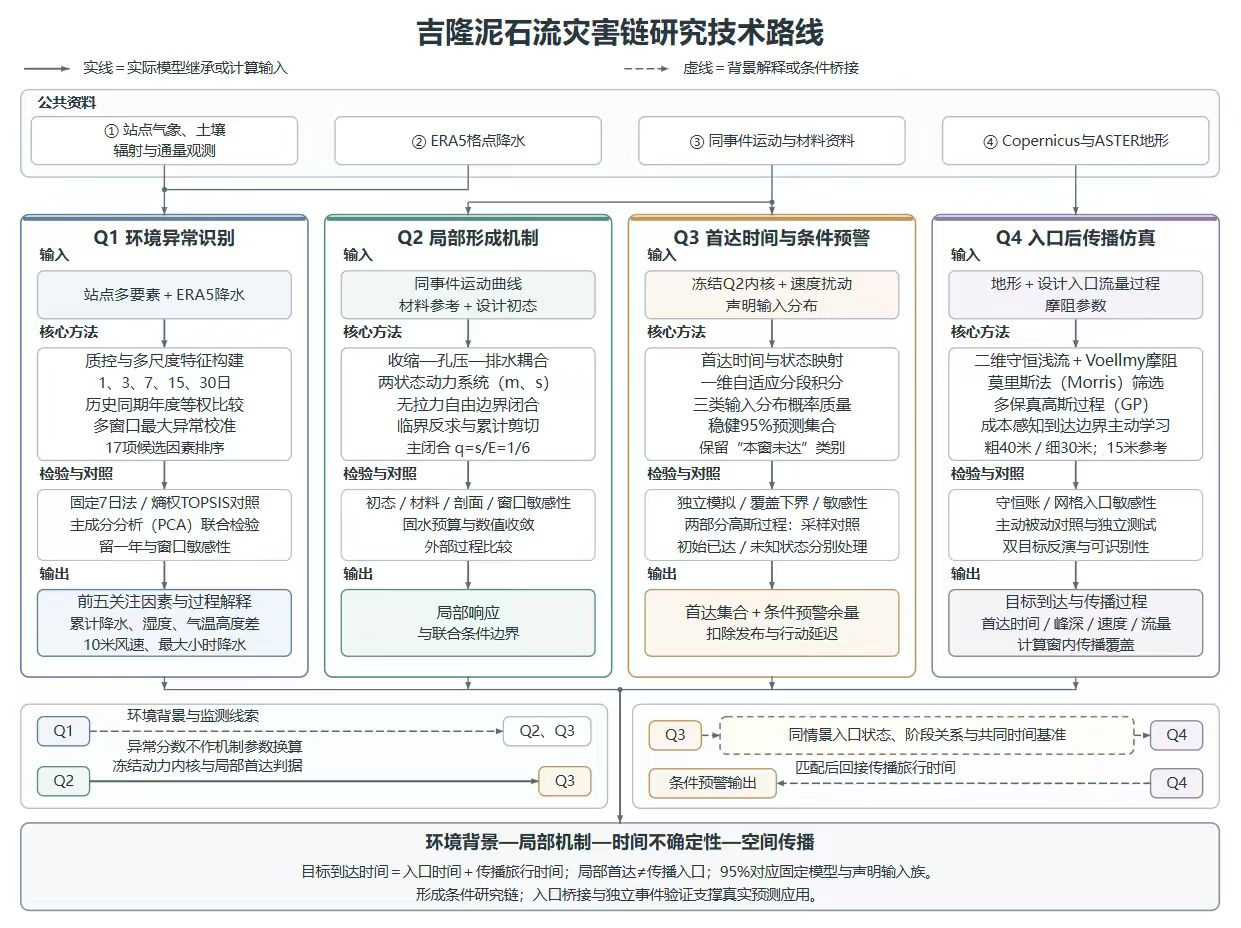
\includegraphics[width=\textwidth]{figures/four_question_roadmap.jpg}
\caption{四问研究技术路线（含补充检验）}\label{fig:route}
\end{figure}
\FloatBarrier

\section{模型假设}

\begin{enumerate}
\item 问题一以北京时间2026年8月26日10:00为回溯截止时刻$t_0$。站点主分析按标签$t$对应$[t-1\mathrm{h},t)$的小时均值处理，并比较$[t,t+1\mathrm{h})$及当日00:00截止的情景。ERA5总降水采用标签之前一小时的水当量。
\item 2021—2026年同名观测变量采用相同对象、单位和统计方式。
\item 2021—2025年同季、同钟点记录作为历史背景，各年赋予相同权重。
\item 问题二将局部细粒材料理想化为饱和柱，固定底面积和固体体积，沿坡面法线取厚度平均状态，顶面可交换液水。
\item 问题三沿用问题二材料柱与二次压力剖面，以选定速度窗起点设置初态；假设整条速度曲线受同一偏移，传播示例采用理想常坡和首达到入口的零阶段延时。
\item 问题四以规定的已形成流进入断面为时间零点，采用常密度固定床、初始干床和设计入流。
\end{enumerate}

问题一以单次事件为对象，采用固定截止时刻的回溯比较。

\Needspace{18\baselineskip}
\section{符号说明}
\renewcommand{\thetable}{\arabic{table}}


\begin{table}[htbp]
\centering
\caption{主要符号及含义}\label{tab:1}
\fontsize{9.5}{12}\selectfont
\setlength{\tabcolsep}{4pt}
\begin{tabularx}{\textwidth}{p{39mm}X}
\toprule
符号 & 含义 \\
\midrule
$j,w,t_0$ & 因素、窗口长度及目标截止时刻 \\
$P_i,P_d,A_d$ & 格点第$i$小时总降水量、截止对齐第$d$日块总降水量及第$d$块前期总降水指数，单位均为mm \\
$X_{j,w}(t)$ & 端点$t$之前窗口$w$内的因素统计量 \\
$W_j$ & 因素$j$固定适用的窗口集合 \\
$B_{j,y},Y_j$ & 年$y$的合格历史端点集、因素$j$的有效历史年集合 \\
$R,h$ & 三参考年集合、留出的校准年 \\
$F^{\mathrm{mid}},q$ & 经验中秩分布、年度等权历史分位位置 \\
$a,M,S$ & 双侧异常、多窗最大异常、历史校准位置 \\
$z,P_k,\Lambda_k$ & 标准化向量、保留主成分矩阵及特征值矩阵 \\
$T^2,Q$ & 保留空间距离、重构残差平方和 \\
$m,H,s$ & 问题二的固相体积分数（无量纲）、柱厚（m）及平均有效法向应力（Pa）；问题一的$H$另指感热通量 \\
$q_0,\chi,\Gamma_{\rm sh}$ & 问题二初始应力比$s_{\rm init}/E$（无量纲）、剪切传递系数（m$^{-1}$）及累计剪切（无量纲）；$E$为浮重法向应力尺度（Pa） \\
$\tau_L,d,a$ & 问题三局部首达时间（s）、整条速度曲线的偏移及偏移支持半宽（m/s） \\
$d_{\rm pub},d_{\rm act}$ & 窗起点至发布的延迟、发布后的行动历时（s） \\
$T_{\rm in},T_A,L_L,L_A$ & 传播入口时刻、目标到达时刻、局部及目标行动余量（s） \\
$h,\mathbf u,z$ & 问题四竖直流深（m）、水平平均流速（m/s）和固定床高（m） \\
\bottomrule
\end{tabularx}
\end{table}

\renewcommand{\thetable}{1-\arabic{table}}
\setcounter{table}{0}
\Needspace{16\baselineskip}
\section{模型建立与求解}

\subsection{问题一}

\questionline{第一问：结合站点逐小时记录与格点总降水，分析事件前区域环境过程，识别相对历史同期突出的五项特征。}

\subsubsection*{1）模型的准备}

采用吉隆综合观测站的气象、土壤、辐射和湍流逐小时记录\cite{ref2}。站点位于28.86°N、85.29°E，海拔约4140 m，距受影响口岸约65 km；观测包括1—20 m气温与标量风速、2 m相对湿度及气压，0.1、0.2、0.4、0.8和1.6 m土壤温度（℃）与体积含水量（m³/m³），以及0.1 m和0.2 m板热流。Rsd和Rld分别为短波与长波辐射原通道，H和LE为感热与潜热通量原通道，单位均为W/m²；USTAR为摩擦速度类原通道（m/s）。2021—2026年小时总降水取ERA5同一最近格点\cite{era5api}：28.75°N、85.25°E、地形高程4756 m、约0.25°分辨率，关闭高程降尺度；总降水为雨雪水当量。

站点数据保留原时间位置与缺测，有质量标记的变量采用质量标记为0的记录，剔除不可解析值、非有限值及缺测标记9999.9。物理范围为摄氏温度高于−273.15 ℃、MET气压为正、土壤体积含水量在[0,1]；时间标签须可解析、唯一并符合所属年份及小时网格。辐射与通量采用原通道及符号\cite{ref3}。

长度为$w$日的回溯窗口覆盖截止前$24w$小时。站点主情景将标签$t$记为$[t-1\mathrm h,t)$的小时均值；ERA5标签为此前一小时总降水，纳入$t_0-24w\mathrm h<t\le t_0$的记录。末7日为8月19日10:00至8月26日10:00，末30日为7月27日10:00至8月26日10:00。

\Needspace{6\baselineskip}
\noindent\hspace*{2em}\topic{近地层结构与灾前过程}

8月26日09:00—10:00的小时均温在1—20 m由12.05 ℃降至11.24 ℃；标量风速随高度变化（图~\ref{fig:1}）。20 m与2 m共同有效小时的30日平均温差为−0.497 ℃，较历史同期偏高。

\begin{figure}[htbp]
\centering
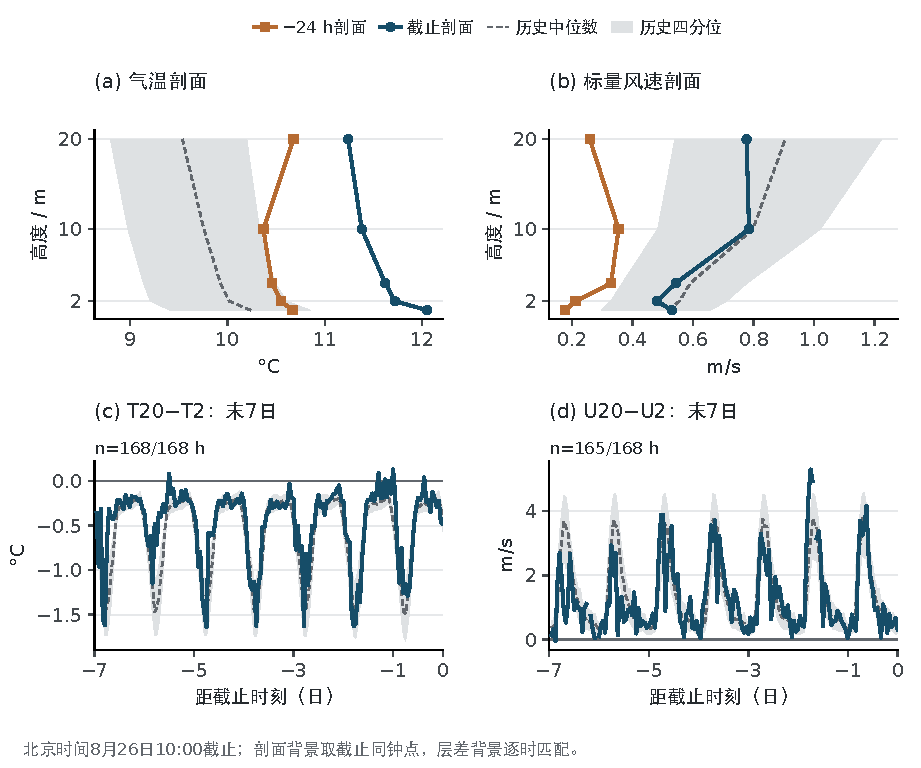
\includegraphics[width=156mm,trim=0 18 0 0,clip]{figures/q1_new/q1_fig01_structure.pdf}
\caption{近地层剖面与配对层间差。上排为截止时刻和提前24 h时刻的两个气温、标量风速剖面，灰带为历史同期、同钟点记录的年度等权四分位范围。下排T20−T2、U20−U2分别为\mbox{20 m减2 m}的气温差与标量风速差；n表示两高度同一小时共同有效的小时数／应有小时数，缺测保留断线。}\label{fig:1}
\end{figure}
\FloatBarrier

\important{长期背景与临近变化并不相同}：30日相对湿润的背景下，末7日出现升温和相对湿度下降（图~\ref{fig:2}）。2 m气温末7日均值为12.51 ℃，首、末24 h均值由11.88 ℃升至13.78 ℃；相对湿度30日均值为71.25\%，末24 h为60.49\%。末7日首末日块中，0.1 m和0.2 m土壤体积含水量均值下降，0.1—0.4 m土温均值上升，0.8 m和1.6 m土温均值略降。

图~\ref{fig:2}以三角标记逐小时历史分位数：对每个过程小时，汇集2021—2025年相应历日前后15日的同钟点记录，逐年等权确定第5和第95百分位；气温分别用两阈值标记偏冷、偏热，风速用第95百分位标记相对强风。

\begin{figure}[htbp]
\centering
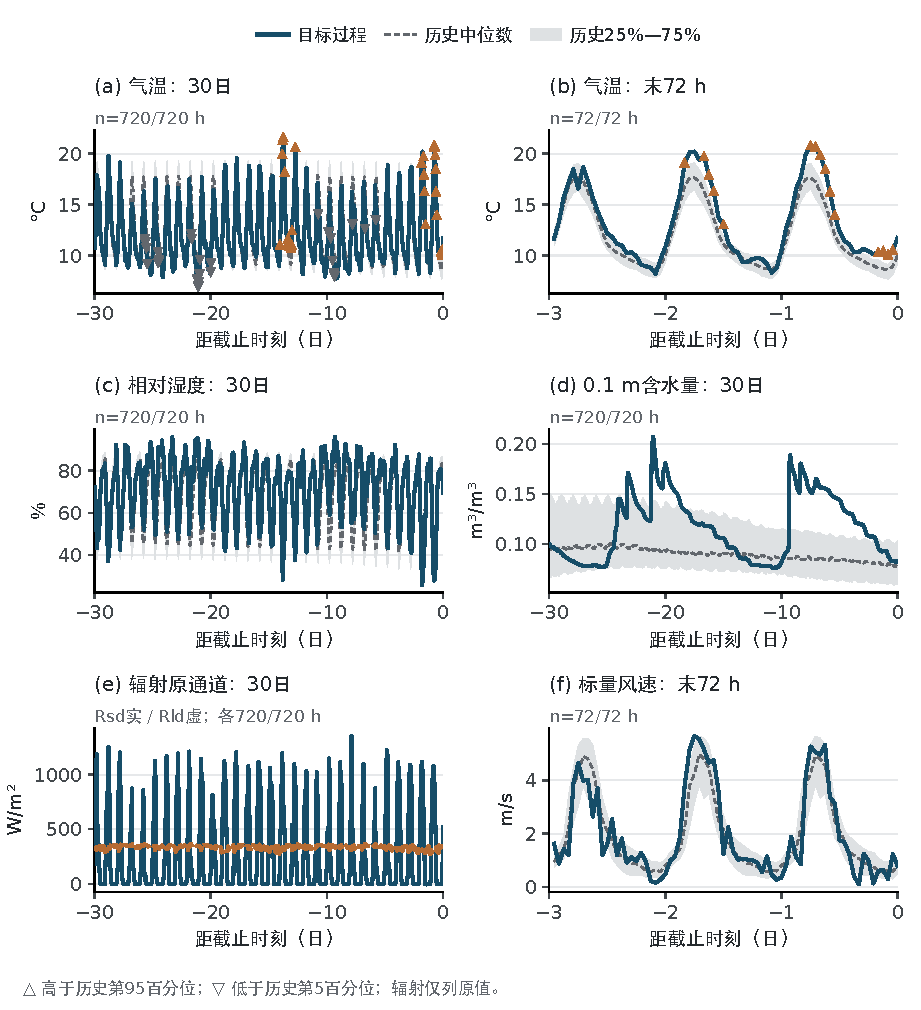
\includegraphics[width=156mm,trim=0 18 0 0,clip]{figures/q1_new/q1_fig02_process.pdf}
\caption{灾前天气与水热过程。展示30日温湿、水分及辐射过程，并与末72 h气温、风速局部对照；历史背景为同期、同钟点的年度等权分布。三角符号标出相对极端的气温或风速时刻；n表示各通道有效小时数／应有小时数。辐射展示原观测通道。}\label{fig:2}
\end{figure}
\FloatBarrier

10 m风速30日均值为1.70 m/s，末72 h均值为2.01 m/s。末7日首末24 h的Rsd、Rld、H和LE均值分别变化约+115.20、−27.66、+21.52和−23.25 W/m²，与同期升温及湿度下降共同呈现。

按逐时阈值，30日内2 m气温有30小时高于第95百分位、28小时低于第5百分位；末7日15个高温超阈小时均在末72 h，10 m风速末72 h无高于第95百分位的小时。

ERA5格点30日、7日及末72 h累计总降水分别为195.7、26.9和5.1 mm（图~\ref{fig:q1precip}）。逐小时第95百分位以2021—2025年相应历日前后15日同钟点记录按年度等权确定；30日、7日及72 h分别有48/720、1/168和0/72小时超过该阈值。

\begin{figure}[htbp]
\centering
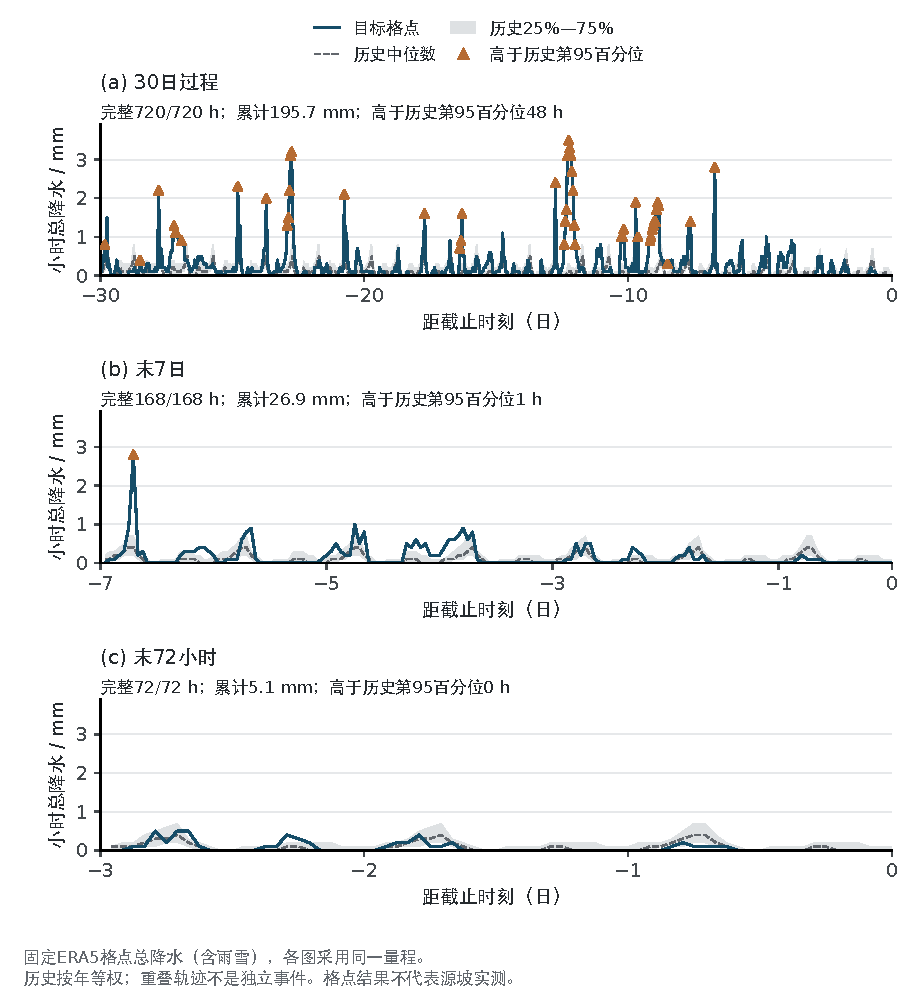
\includegraphics[width=156mm,trim=0 26 0 0,clip]{figures/q1_new/q1_fig03_precipitation.pdf}
\caption{ERA5格点小时总降水过程与历史第95百分位。分别展示30日、7日和72 h；降水为雨雪水当量，阈值由2021—2025年记录构造。}\label{fig:q1precip}
\end{figure}
\FloatBarrier

\begin{table}[htbp]
\centering
\caption{ERA5格点总降水五窗口统计量。最大小时量除以1 h为小时平均率，有降水小时按单小时总量不小于0.1 mm计。}\label{tab:q1precip}
\fontsize{9.5}{12}\selectfont
\setlength{\tabcolsep}{4pt}
\begin{tabularx}{\textwidth}{*{5}{>{\centering\arraybackslash}X}}
\toprule
窗口 & 累计/mm & 最大小时总量/mm & 有降水小时/h & 前期指数/mm \\
\midrule
1日 & 0.7 & 0.2 & 6 & 0.700 \\
3日 & 5.1 & 0.5 & 25 & 4.381 \\
7日 & 26.9 & 2.8 & 74 & 17.920 \\
15日 & 102.5 & 3.5 & 212 & 43.821 \\
30日 & 195.7 & 3.5 & 471 & 53.203 \\
\bottomrule
\end{tabularx}
\end{table}
\FloatBarrier

\subsubsection*{2）模型的建立}

\noindent\hspace*{2em}\topic{因素定义与历史样本}

采用17项候选（表~\ref{tab:2}），包含格点降水、站点热力、辐射、浅土、层间差及常规天气量。窗口内最大小时均温为$\max_i T_i$，$T_i$为该窗第$i$小时的2 m均温。


\begin{table}[htbp]
\centering
\caption{17项候选因素的物理分类}\label{tab:2}
\fontsize{9.5}{12}\selectfont
\setlength{\tabcolsep}{4pt}
\begin{tabularx}{\textwidth}{p{33mm}X}
\toprule
物理类别 & 具体变量、统计量及单位 \\
\midrule
格点降水（4项） & 累计总降水、最大小时总量、前期总降水指数（mm）；有降水小时数（h） \\
近地热力（3项） & 正温指数（℃·h）；最大小时均温（℃）；24 h块均温变化率（℃/d） \\
辐射（2项） & Rsd、Rld原通道均值（W/m²） \\
浅土水热（3项） & 0.1 m体积含水量均值（m³/m³）、土温均值（℃）、板热流均值（W/m²） \\
近地层结构（2项） & 20 m−2 m气温差均值（℃）及标量风速差均值（m/s） \\
常规天气（3项） & MET气压均值（hPa）、2 m相对湿度均值（\%）、10 m标量风速均值（m/s） \\
\bottomrule
\end{tabularx}
\end{table}

均值、PDD和最大小时均温采用1、3、7、15、30日窗口，均温变化率使用3日及以上窗口。站点均值要求有效小时达到全窗90\%，PDD、最大小时均温及四项格点降水要求全窗完整。

\important{正温指数PDD}按$\sum_i\max(T_i,0)\Delta t$计算，$\Delta t=1\mathrm h$，单位℃·h。均温变化率以截止对齐的24 h合格块均温对实际时间线性拟合，斜率单位℃/d；主设置要求每块至少22小时有效、全窗有效小时和合格块均不少于90\%，至少3块且首末块合格。

设$P_i$为ERA5前一小时总降水量（mm），四项统计量为累计量$\sum_iP_i$、最大小时量$\max_iP_i$、$P_i\ge0.1$ mm的小时数及前期总降水指数。后者将窗口分成截止对齐的24 h块并按时间由早到晚编号，首块前$A_0=0$，按$A_d=P_d+0.9A_{d-1}$递推；$P_d$为第$d$块总降水，指数单位为mm，日衰减系数0.9无量纲。每个窗口均从零开始；2.8 mm的小时总量折合小时平均率2.8 mm/h。

\Needspace{7\baselineskip}
两项高度差先在同一小时的两层记录共同有效时作差，再求窗口均值：

\[
\Delta T(t)=T_{20\mathrm{m}}(t)-T_{2\mathrm{m}}(t),\qquad
\Delta U(t)=U_{20\mathrm{m}}(t)-U_{2\mathrm{m}}(t).
\tag{1}
\]

式（1）中$T$和$U$分别为所标高度的气温和标量风速；差值单位分别为℃和m/s。

同期背景取2021—2025年各年8月26日前后15日、与截止同钟点的31个候选端点。对因素$j$，端点的全部适用窗口$W_j$均须有效；每年至少保留25个端点，且至少4年合格，目标采用相同的窗口集合。

\noindent\hspace*{2em}\topic{年度等权的多尺度历史校准}

依次计算实际统计量、单窗历史位置$q$、双侧择窗结果$M$与留出年校准位置$S$：先将窗口统计值与三参考年同期记录比较，得到$q$；再取该因素适用窗口中的最大双侧异常$M$；最后用留出历史端点的$M$分布确定目标位置$S$。每次留出一年$h$作为\important{校准年}，从其余有效年中选三年组成参考集合$R$，记一组配置为$(h,R)$。

\Needspace{9\baselineskip}
记$B_{j,y}$为因素$j$在年$y$的合格端点集，$n_{j,y}$为端点数，$u$为历史端点，$x$为待比较的窗口统计值。指示函数$\mathbf{1}_{\{C\}}$在条件$C$成立时取1，否则取0；中秩将小于$x$的端点计1、等于$x$的端点计1/2。年内经验分布为

\[
F^{\mathrm{mid}}_{j,w,y}(x)=\frac{1}{n_{j,y}}
\sum_{u\in B_{j,y}}\left[\mathbf{1}_{\{X_{j,w}(u)<x\}}+
\tfrac12\mathbf{1}_{\{X_{j,w}(u)=x\}}\right].
\tag{2}
\]

\Needspace{6\baselineskip}
对三参考年的年内位置取等权平均，得到端点$t$在窗口$w$上的历史分位位置

\[
q_{j,w,R}(t)=\frac13\sum_{y\in R}
F^{\mathrm{mid}}_{j,w,y}\bigl(X_{j,w}(t)\bigr).
\tag{3}
\]

$q$接近1表示高于大多数同期记录，接近0表示偏低，接近0.5表示居中。将$q$距中间位置的程度记为双侧异常$a$，在固定窗口集合中取最大值$M$：

\[
a_{j,w,R}(t)=\left|2q_{j,w,R}(t)-1\right|,\qquad
M_{j,R}(t)=\max_{w\in W_j}a_{j,w,R}(t).
\tag{4}
\]

对目标与留出校准年的所有端点均执行式（4）；并列的最大异常窗口全部保留。

\Needspace{6\baselineskip}
记$F^{\mathrm{mid}}_{M,j,h,R}$为留出年$h$各合格端点的多窗最大异常$M$构成的中秩分布，$\mathcal R_{j,h}$为该校准年对应的合法三参考年集合，则历史校准位置为

\[
S_j=\frac1{|Y_j|}\sum_{h\in Y_j}
\frac1{|\mathcal R_{j,h}|}\sum_{R\in\mathcal R_{j,h}}
F^{\mathrm{mid}}_{M,j,h,R}\bigl(M_{j,R}(t_0)\bigr).
\tag{5}
\]

式中$|Y_j|$为有效校准年数，$|\mathcal R_{j,h}|$为对应的三参考年集合数。五个有效年形成20个参考—校准配置，四年形成4个。$S$先在同一校准年内对参考集合平均，再对校准年等权平均；$S$越大，目标最大异常在历史背景中越突出。

对物理信息重复的候选，采用7日窗、至少4个共同有效年及每年至少25个配对端点；历史Spearman秩相关绝对值达到0.90时合并。均温与PDD的相关为1且$S$相同，保留PDD代表。

\subsubsection*{3）模型的求解与分析}

\noindent\hspace*{2em}\topic{关注排序与过程解释}

五项关注特征依次为ERA5格点累计总降水、2 m相对湿度均值、20 m−2 m气温差均值、10 m标量风速均值及ERA5格点最大小时总降水量，$S$分别为0.902、0.869、0.854、0.852和0.845（表~\ref{tab:3}）。$S$综合全部适用窗口；表中主要窗口为参考—校准配置中达到最大双侧异常频次最高的窗口，并列最大均计数。四项主要窗口为30日、最大小时量为7日。


\begin{table}[htbp]
\centering
\caption{前五关注特征及主要窗口}\label{tab:3}
\fontsize{9.5}{12}\selectfont
\setlength{\tabcolsep}{4pt}
\begin{tabularx}{\textwidth}{p{43mm}r c c X}
\toprule
关注特征 & $S$ & 主要窗口 & 目标值 & 该窗平均$q$及方向 \\
\midrule
ERA5格点累计总降水 & 0.902 & 30日 & 195.7 mm & 0.994，偏高 \\
2 m相对湿度均值 & 0.869 & 30日 & 71.25\% & 1.000，偏高 \\
20 m−2 m气温差均值 & 0.854 & 30日 & −0.497 ℃ & 1.000，偏高 \\
10 m标量风速均值 & 0.852 & 30日 & 1.70 m/s & 0.000，偏低 \\
ERA5格点最大小时总降水量 & 0.845 & 7日 & 2.8 mm & 1.000，偏高 \\
\bottomrule
\end{tabularx}
\end{table}

\begin{figure}[htbp]
\centering
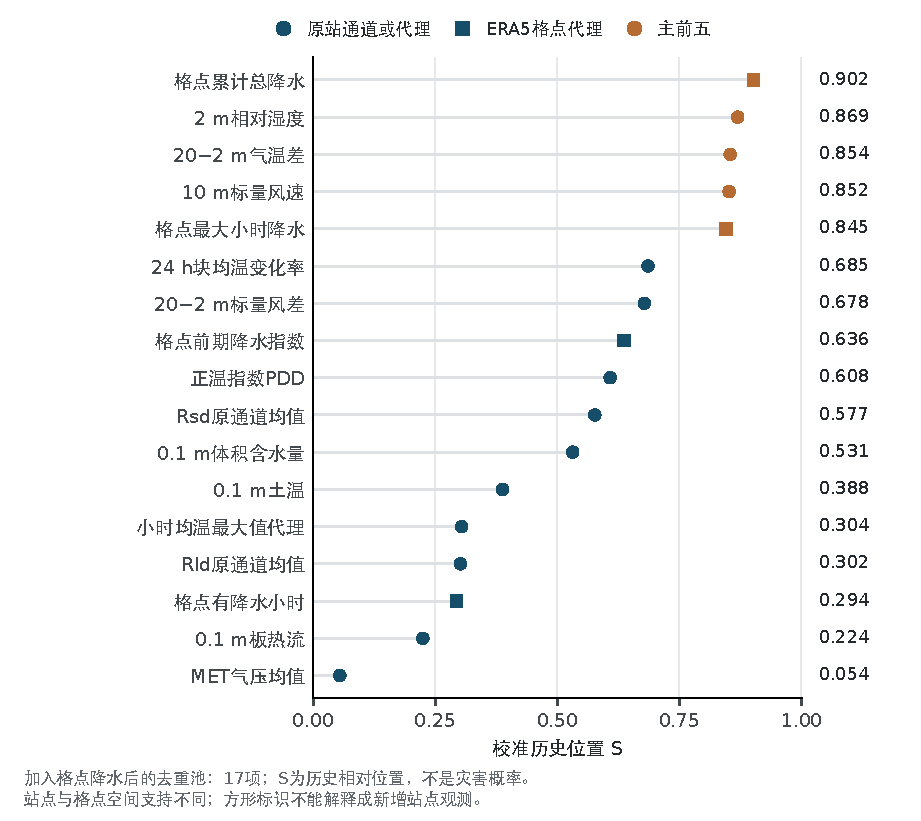
\includegraphics[width=156mm,trim=0 26 0 0,clip]{figures/q1_new/q1_fig04_ranking.pdf}
\caption{17项候选的历史校准位置。颜色区分前五与其余候选，形状区分站点变量与格点表达；$S$为历史校准位置。图中“小时均温最大值代理”对应窗口内最大小时均温。}\label{fig:3}
\end{figure}
\FloatBarrier

\important{降水的历史位置随尺度分化}：30日累计195.7 mm、15日102.5 mm的平均$q$分别为0.994和0.981，均偏高；末24 h和72 h累计0.7 mm、5.1 mm，平均$q$为0.084和0.158，均偏低。7日最大小时量为2.8 mm，平均$q=1$；末24 h和72 h的最大值分别为0.2和0.5 mm。站点30日相对湿度亦偏高，而末24 h与72 h平均$q$分别为0.168和0.252。

气温高度差30日均值为−0.497 ℃，较历史同期偏高；末7日首末24 h均值由−0.429 ℃变为−0.520 ℃。10 m风速30日位置偏低，3日平均$q=0.510$；3日标量风速高度差的方向随参考配置变化。

均温变化率的7日斜率为+0.349 ℃/d，末72 h为+0.552 ℃/d；7日单窗双侧异常为0.897，多窗历史校准位置为0.685。

\Needspace{6\baselineskip}
\noindent\hspace*{2em}\topic{敏感性分析}

为考察前五特征对分析设置和历史年份的依赖，比较11种时间、完整性、窗口及历史支持设置，并逐次剔除一个历史年；表~\ref{tab:5}给出各设置的入选和可评分次数。

\begin{table}[htbp]
\centering
\caption{前五特征对分析设置和历史年份的敏感性}\label{tab:5}
\fontsize{9.5}{12}\selectfont
\setlength{\tabcolsep}{4pt}
\begin{tabularx}{\textwidth}{p{30mm}*{4}{>{\centering\arraybackslash}X}}
\toprule
特征 & 11种设置的$S$范围 & 设置入选/可算 & 逐年剔除入选/可算 & 逐年剔除名次范围 \\
\midrule
格点累计总降水 & 0.856—0.902 & 11/11 & 5/5 & 1—2 \\
相对湿度 & 0.670—0.874 & 10/11 & 5/5 & 2—5 \\
气温高度差 & 0.685—0.857 & 10/11 & 5/5 & 1—5 \\
10 m标量风速 & 0.315—0.853 & 10/11 & 5/5 & 3—5 \\
格点最大小时量 & 0.844—0.918 & 11/11 & 5/5 & 1—5 \\
\bottomrule
\end{tabularx}
\end{table}
\FloatBarrier

11种设置涵盖站点时标、截止时刻、覆盖率、窗口、历史端点及去重阈值，并比较共同历史支持；后者取合并重复温度信息前18项可评分因素的适用窗口均有效的历史端点。“入选／可算”为进入前五的次数与可评分次数之比。

五项在5次逐年剔除中均保留；删除30日窗后，前五变为格点最大小时量、格点累计量、PDD、均温变化率和Rsd。

\noindent\hspace*{2em}\topic{多变量联合结构核验}

为判断各因素共同出现时是否偏离历史，将同一窗口的17个实际统计量组成向量，分别在7日和30日开展主成分分析（PCA）。每行对应一个历史端点，两个尺度共用148个完整端点，2021—2025年依次为31、31、31、26、29行。每个参考—校准配置用三参考年按年等权拟合中心、标准差和协方差；年$y$有$n_y$个端点时，每行权重为$1/(3n_y)$，目标与校准年应用同一组参数。

保留成分数$k$取累计解释方差首次达到85\%的最小值：7日模型$k=5$或6，30日模型$k=3$或4；合法的$k-1$和$k+1$另作敏感性比较。

设$x_j$为该窗口的第$j$项统计量，$\mu_j$和$\sigma_j$为三参考年的加权中心和标准差，$z_j=(x_j-\mu_j)/\sigma_j$为标准化后的第$j$项，$z$为所得17维列向量，$P_k$的列为保留的$k$个单位正交主成分方向，$\Lambda_k$为对应特征值组成的对角矩阵；上标$\mathsf T$表示转置。

\Needspace{7\baselineskip}
用保留空间中的距离$T^2$和重构残差平方和$Q$分别描述联合偏离：

\[
T^2=z^{\mathsf T}P_k\Lambda_k^{-1}P_k^{\mathsf T}z,\qquad
e=z-P_kP_k^{\mathsf T}z,\qquad Q=e^{\mathsf T}e.
\tag{6}
\]

$T^2$衡量沿历史共同变化方向的标准化距离；$e$是原标准化向量减去保留成分重构值后得到的残差，$Q$为残差平方和，衡量未被保留成分解释的偏离\cite{ref7}。分别将目标的两量与同一模型的校准年比较，求其中秩位置，再依式（5）先平均同一校准年的参考组合、后跨年等权汇总。两量分别比较。


\begin{table}[htbp]
\centering
\caption{PCA联合指标在留出背景中的历史位置}\label{tab:6}
\fontsize{9.5}{12}\selectfont
\setlength{\tabcolsep}{4pt}
\begin{tabularx}{\textwidth}{*{5}{>{\centering\arraybackslash}X}}
\toprule
尺度 & $T^2$汇总位置 & $T^2$组合范围 & $Q$汇总位置 & $Q$组合范围 \\
\midrule
7日 & 0.677 & 0.069—1.000 & 0.628 & 0.161—1.000 \\
30日 & 0.745 & 0.231—1.000 & 0.142 & 0—0.806 \\
\bottomrule
\end{tabularx}
\end{table}

\begin{figure}[htbp]
\centering
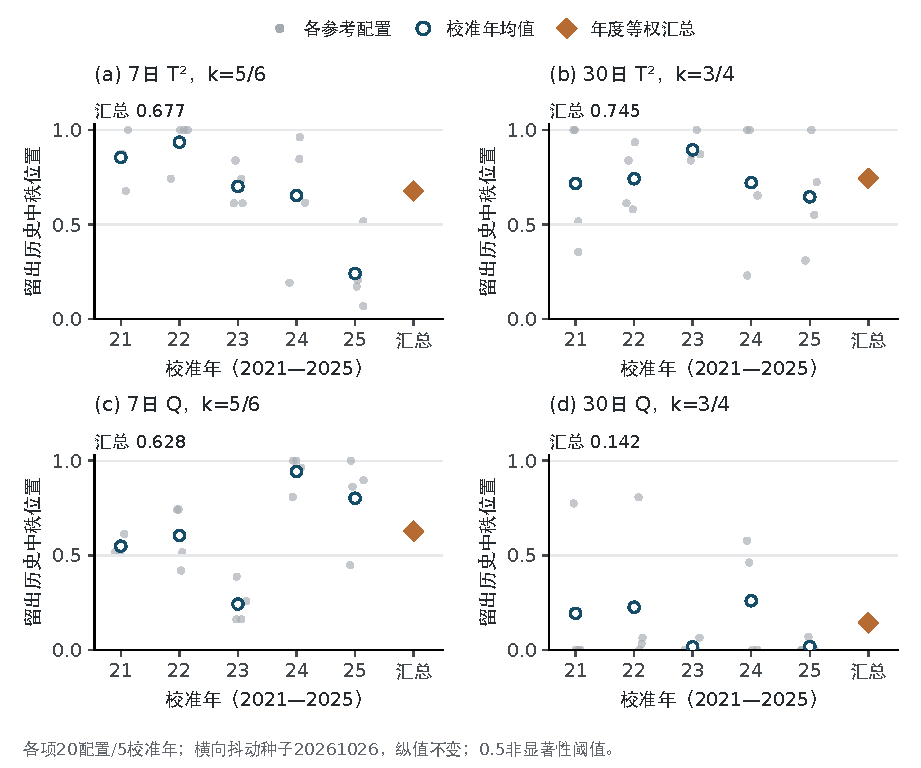
\includegraphics[width=156mm,trim=0 18 0 0,clip]{figures/q1_new/q1_fig05_pca.pdf}
\caption{两个固定尺度的17项联合历史位置。展示各参考组合、校准年均值和年度等权汇总；散点横向错位用于区分不同配置。7日$k$取5或6，30日取3或4。}\label{fig:4}
\end{figure}
\FloatBarrier

联合位置随参考年份组合变化（表~\ref{tab:6}、图~\ref{fig:4}）；改变成分数后，7日和30日$T^2$汇总位置分别为0.677—0.739和0.677—0.816。

\Needspace{6\baselineskip}
为定位各变量的联合偏离，将$T^2$和$Q$分解为可相加的原变量项：

\[
c_j^T=z_j\bigl[P_k\Lambda_k^{-1}P_k^{\mathsf T}z\bigr]_j,
\qquad c_j^Q=e_j^2,
\qquad \sum_jc_j^T=T^2,\quad\sum_jc_j^Q=Q.
\tag{7}
\]

式中方括号下标$j$表示向量的第$j$个分量，$c_j^T$和$c_j^Q$为因素$j$对$T^2$和$Q$的可加项；对非零的对应统计量，各模型分别计算$c_j^T/T^2$和$c_j^Q/Q$，先对同一校准年的参考集合平均，再对校准年等权平均。$T^2$的有符号分解允许个别份额为负。7日距离中均温变化率和浅层含水量份额较大，残差中最大小时总降水量份额较大；30日距离中累计降水、湿度及高度差等份额较大。

\Needspace{12\baselineskip}
\subsection{问题二}
\renewcommand{\thefigure}{2-\arabic{figure}}\setcounter{figure}{0}
\renewcommand{\thetable}{2-\arabic{table}}\setcounter{table}{0}
\questionline{第二问：建立饱和细粒基质的孔压反馈模型，分析初始状态与累计剪切共同决定的起始条件。}

\subsubsection*{1）模型的准备}

\noindent\hspace*{2em}\topic{研究对象和输入资料}

问题二研究吉隆冰崩—泥石流灾害链的触发与物质转化条件。此次“8·26”灾害链源于蓝塘里壤峰高位冰岩崩：冰岩体撞击错坚河谷底后，运动物质裹挟冰川冰和湿细粒冰碛物，沿错坚河下行至普热普藏布\cite{q2yin}。本文据此研究湿细粒冰碛物受剪时的孔压变化，将其中细颗粒与孔隙水理想化为单位平面面积的饱和材料柱：柱厚沿坡面法线方向，固体体积固定，基底不透水，顶面可交换液水；以固相体积分数和厚度平均有效法向应力描述柱体状态。

颗粒骨架受剪收缩、孔隙水排出滞后时，孔隙水压力（孔压）上升，颗粒承担的接触应力降低；排水则缓解这一变化。柱上部接触应力降至零时，孔压承担法向荷载；零接触应力区域开始具有正厚度的边界称为\important{孔压支承层起始条件}。

由撞击谷底至错坚河沟口的8个地图顶点得到平面折线长度约5.37 km；以两端高程3900、3020 m的差值除以该长度并取反正切，得平均坡度$\theta=9.31^\circ$\cite{q2yin}，用于法向浮重计算。同文纵剖面的另一组距离和高差给出8.51°，用于几何敏感性比较。

外部速度$U_{\mathrm{ext}}$采用同事件地震信号反演的整体沿坡速度，按图中约5 s间隔读点线性插值，读取范围约为$\pm1.5$ m/s\cite{q2yin}。取源释放后27—100 s的曲线驱动材料柱，模型时间$t=0$对应相对27 s，窗长73 s。速度积分表示外部累计运动尺度。

图~\ref{fig:q2input}展示运动输入及瑞士Blatten冰岩崩沉积物的细粒样本。采用文献报告的饱和导水率均值$K_{fs}=1.5\times10^{-5}$ m/s\cite{q2kang,q2data}，以清水动力黏度$\mu_w=0.001$ Pa·s和水密度$\rho_w=1000$ kg/m³换算，得到初始渗透率$k_i=K_{fs}\mu_w/(\rho_w g)=1.529\times10^{-12}$ m²；模型另取细粒悬液有效黏度$\mu=0.01$ Pa·s。



\begin{figure}[htbp]
\centering
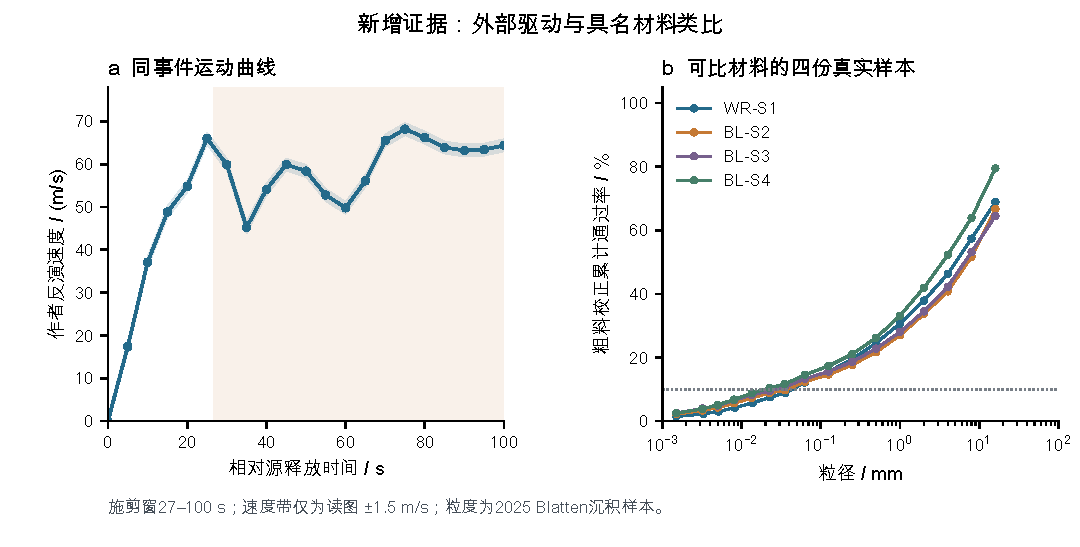
\includegraphics[width=152mm,trim=0 24 0 20,clip]{figures/q2/fig01_new_evidence.pdf}
\caption{反演运动输入与Blatten沉积物粒度。速度包络表示图示读取范围；右图为四个细粒样本。}\label{fig:q2input}
\end{figure}
\FloatBarrier

\Needspace{6\baselineskip}
\noindent\hspace*{2em}\topic{初态与工作假设}

设计初态取固相体积分数$m_0=0.54$、柱厚$H_0=1$ m和初始有效应力比$q_0=0.17,0.30,0.50,0.75$；强施剪情景取$\chi=0.02$ m$^{-1}$。材料参数取临界固相分数$m_{\rm crit}=0.60$、无量纲压缩性参数$a_c=0.03$、应力正则量$\sigma_0=100$ Pa、颗粒碰撞长度尺度$\delta=0.001$ m和固体密度$\rho_s=2700$ kg/m³\cite{q2iverson14}。

\subsubsection*{2）模型的建立}

\noindent\hspace*{2em}\topic{状态、本构与外部剪切}

记$m$为固相体积分数（无量纲），$H$为沿坡面法线的柱厚（m），$s$为厚度平均有效法向应力（Pa），即扣除孔压后颗粒骨架承担的法向应力。单位面积固体体积$H_s=m_0H_0=mH$，固体浮重的法向应力尺度为$E=(\rho_s-\rho_w)g\cos\theta H_s$（Pa），其中$g=9.81$ m/s²。固定固体体积与坡度下$E$为常数，$H$由$m$恢复；静水孔压时$s=E/2$。初始值$s_{\rm init}=q_0E$，因此$q_0=0.50$是初始超孔压为零的参考状态。

源模型的平均有效应力为$\sigma_e=\operatorname{tr}(T_e)/3$，$T_e$为有效应力张量。以厚度平均法向应力$s$近似替代$\sigma_e$，代入剪胀—压缩性关系\cite{q2iverson14}：
\[
\begin{aligned}
\alpha&=\frac{a_c}{m(s+\sigma_0)},&
N&=\frac{\mu\dot\gamma}{\rho_s\dot\gamma^2\delta^2+s},\\
\tan\psi&=m-\frac{m_{\rm crit}}{1+\sqrt N},&
k&=k_i\exp[(m_0-m)/0.04].
\end{aligned} \tag{8}
\]
式中$\alpha$为压缩性（Pa$^{-1}$），$N$为无量纲黏性数，$\psi$为剪胀角，$k$为渗透率（m²），$\dot\gamma$为剪切率（s$^{-1}$）；$\dot\gamma=0$时取$N=0$。$m$与经$N$修正的临界分数比较决定$\tan\psi$的符号：负值表示收缩，正值表示剪胀。$a_c$控制压缩性，$\sigma_0$避免低应力时压缩性发散，$\delta$决定颗粒碰撞应力的长度尺度。渗透率以初态$m_0$的初始值$k_i$为锚点；指数中的0.04为无量纲固相分数尺度，控制渗透率对固相分数变化的敏感程度，取自源经验关系\cite{q2iverson14}。$\chi$综合局部滑移、受剪尺度与应变分配，将整体速度映射为局部剪切率，单位为m$^{-1}$：
\[
\dot\gamma(t)=\chi U_{\mathrm{ext}}(t+27\,\mathrm{s}),\qquad 0\le t\le73\,\mathrm{s}. \tag{9}
\]

\noindent\hspace*{2em}\topic{无拉力分层与水量平衡}

取沿坡面法线自基底向上的坐标$z$（m），令$x=z/H$；$p_e$为相对静水分布的超孔压（Pa），$e=p_e(0)$为基底超孔压，$J$为向上的等效Darcy通量（m/s）。基底不透水，顶面超孔压为零。采用二次超孔压剖面\cite{q2iverson14}，由平均有效应力得到基底超孔压和顶面通量；未分层时有
\[
e=\tfrac32(E/2-s),\qquad p_e(x)=e(1-x^2),\qquad J=\frac{2ke}{\mu H},\qquad s/E\ge\tfrac16. \tag{10}
\]
当二次剖面的上部接触应力降至零后，令$0<s/E<1/6$，并设$r=\sqrt{6s/E}$、$f=1-r$为孔压支承层厚度占比。本文采用无拉力分层及相应等效Darcy通量，得到
\[
e=E(1-r/2),\quad J=\frac{kE}{\mu H},\quad
p_e(x)=\begin{cases}e-Ex^2/(2r),&0\le x\le r,\\E(1-x),&r<x\le1.\end{cases} \tag{11}
\]
总孔压为$\rho_wg\cos\theta H(1-x)+p_e$；式（11）中下部接触应力为$E(r-x)^2/(2r)$，上部为零，其深度平均为$s=Er^2/6$。两支在$r=1$处压力、梯度和通量连续，因此$q_c=s/E=1/6$是本剖面的支承层起始边界；等号处$f=0$，继续越过才有正厚度支承层。

由固体守恒、饱和体积预算及式（8）的本构关系得到，其中上点表示对模型时间$t$求导：
\[
\dot m=\frac{mJ}{H},\qquad
\dot s=\frac{\dot\gamma\tan\psi+J/H}{\alpha},\qquad
\dot H=-J. \tag{12}
\]
$J<0$表示顶面吸水，依赖外部供水；$J>0$表示排水，使柱厚减小、固相分数增大。式（12）中剪切收缩项降低$s$，排水项提高$s$，两者共同决定应力变化。一般初态的初始通量$J_0=2k_i e_0/(\mu H_0)$，$e_0=\frac32(E/2-s_{\rm init})$，只有$q_0=0.50$的$J_0$为零。高于静水参考的初始有效应力对应负超孔压；饱和情景要求总孔压非负，达到这一边界时结束该饱和情景。初态工作范围为$1/6<q_0<q_{\max}$，其中
\[
q_{\max}=\frac12+\frac{\rho_w}{3(\rho_s-\rho_w)m_0}\approx0.863108. \tag{13}
\]
四个设计初态均在此范围内。

\Needspace{6\baselineskip}
\noindent\hspace*{2em}\topic{累计剪切与临界反求}

若排水及材料结构变化都较小，收缩导致的应力下降主要由累计剪切决定；以下用数值轨迹检验这一近似。令$I_U(t)=\int_0^t U_{\mathrm{ext}}(\tau+27\,\mathrm{s})\,d\tau$（m），累计剪切$\Gamma_{\rm sh}=\chi I_U$为无量纲量。由式（8）、（12）可积分得到
\[
\ln\frac{s(t)+\sigma_0}{s_{\rm init}+\sigma_0}
=\frac{1}{a_c}\int_0^t m\dot\gamma\tan\psi\,d\tau+\frac{m(t)-m_0}{a_c}. \tag{14}
\]
右侧第一项为剪切贡献，第二项是与排水相关的体变贡献。若到达起始边界前排水弱、$m\simeq m_0$，且$N$对$\Delta=m_{\rm crit}-m_0>0$的修正较小，则
\[
\begin{aligned}
s+\sigma_0&\simeq(s_{\rm init}+\sigma_0)\exp\!\left(-\frac{m_0\Delta}{a_c}\Gamma_{\rm sh}\right),\\
\Gamma_{c,\mathrm{asy}}&=\frac{a_c}{m_0\Delta}\ln\frac{s_{\rm init}+\sigma_0}{q_cE+\sigma_0},\qquad
\chi_{\mathrm{asy}}=\frac{\Gamma_{c,\mathrm{asy}}}{I_U(T)}.
\end{aligned} \tag{15}
\]
式中$T$为规定窗长，$\Gamma_{c,\mathrm{asy}}$与$\chi_{\mathrm{asy}}$分别为近似临界累计剪切和传递系数；要求$s_{\rm init}>q_cE$且$I_U(T)>0$。为检验近似，定义对数目标间隔和排水绝对贡献比
\[
L_{\rm goal}=\ln\frac{s_{\rm init}+\sigma_0}{q_cE+\sigma_0},\qquad
\epsilon_J=\frac{\int_0^{t_{\rm cut}}|mJ/(a_cH)|\,dt}{L_{\rm goal}}, \tag{16}
\]
其中$t_{\rm cut}$为首次到达边界、计算窗结束或越出饱和模型有效域的时刻。$\epsilon_J$衡量排水相对于所需应力下降的量级；在$0\le t\le t_{\rm cut}$上，同时定义无量纲诊断量$\epsilon_m=\max|m-m_0|/\Delta$和$\epsilon_N=\max[m_{\rm crit}\sqrt N/((1+\sqrt N)\Delta)]$，分别衡量固相变化及$N$修正相对于$\Delta$的大小。

固定初态、材料与外部速度，改变$\chi$，在73 s窗内求最小应力恰好触及$q_cE$的条件根：令$G(\chi)=\min_{0\le t\le T}s(t)/E-q_c$，采用Radau积分，并在有效异号区间用Brent法求$G(\chi^*)=0$。

\Needspace{9\baselineskip}
\subsubsection*{3）模型的求解与分析}

\noindent\hspace*{2em}\topic{初态与累计剪切联合边界}

主材料条件与73 s速度窗下，四个初态的临界根、累计剪切及共同施剪响应见表~\ref{tab:q2root}；完整窗速度积分$I_U(73)=4329.44$ m。

共同采用$\chi_{\rm cmp}=2.265378784906\times10^{-4}$ m$^{-1}$时，前三个初态分别在1.21、41.7和72.9971 s到达边界，$q_0=0.75$在73 s内未到。强施剪档$\chi=0.02$ m$^{-1}$下，$q_0=0.50$的到达时间为0.792 s。

\begin{table}[htbp]
\centering
\caption{四个设计初态的临界根与共同比较档响应}\label{tab:q2root}
\fontsize{9.5}{12}\selectfont
\setlength{\tabcolsep}{4pt}
\begin{tabularx}{\textwidth}{*{4}{>{\centering\arraybackslash}X}}
\toprule
$q_0$ & $\chi^*$（m$^{-1}$） & $\chi^*I_U(73)$ & 共同$\chi_{\rm cmp}$首次到边界（s） \\
\midrule
0.17 & $4.35\times10^{-6}$ & 0.0188 & 1.21 \\
0.30 & $1.20\times10^{-4}$ & 0.520 & 41.7 \\
0.50 & $2.27\times10^{-4}$ & 0.981 & 72.9971 \\
0.75 & $3.12\times10^{-4}$ & 1.35 & 73 s内未到达边界 \\
\bottomrule
\end{tabularx}
\end{table}
\begin{figure}[htbp]
\centering
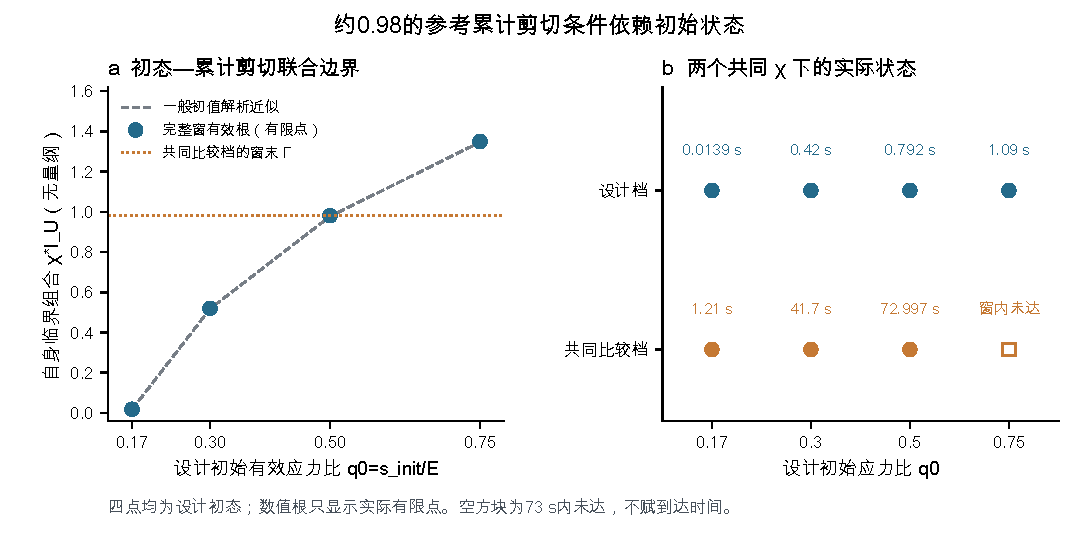
\includegraphics[width=152mm,trim=0 24 0 20,clip]{figures/q2/fig07_initial_state_boundary.pdf}
\caption{四个初态的临界根与共同施剪响应。左图为临界根及近似值，右图比较两档剪切；空方块表示完整规定窗内未到达支承层起始边界。事件时刻由折线输入的数值解给出。}\label{fig:q2root}
\end{figure}
\FloatBarrier

\noindent\hspace*{2em}\topic{排水对近似的影响}

初态接近起始边界时，达到边界所需的应力下降较小，排水相对作用增强。四个初态的临界根相对近似值偏差$(\chi^*-\chi_{\rm asy})/\chi_{\rm asy}$依次为9.66\%、0.482\%、0.347\%和0.289\%。$q_0=0.17$时，略高于临界剪切系数的弱施剪轨迹，其排水绝对贡献占目标对数应力下降的9.54\%；\mbox{同一初态}在共同档$\chi_{\rm cmp}$下为0.159\%；前者固相变化和$N$修正相对$\Delta$分别为$8.86\times10^{-4}$和$4.47\times10^{-4}$（图~\ref{fig:q2diag}）。

\begin{figure}[htbp]
\centering
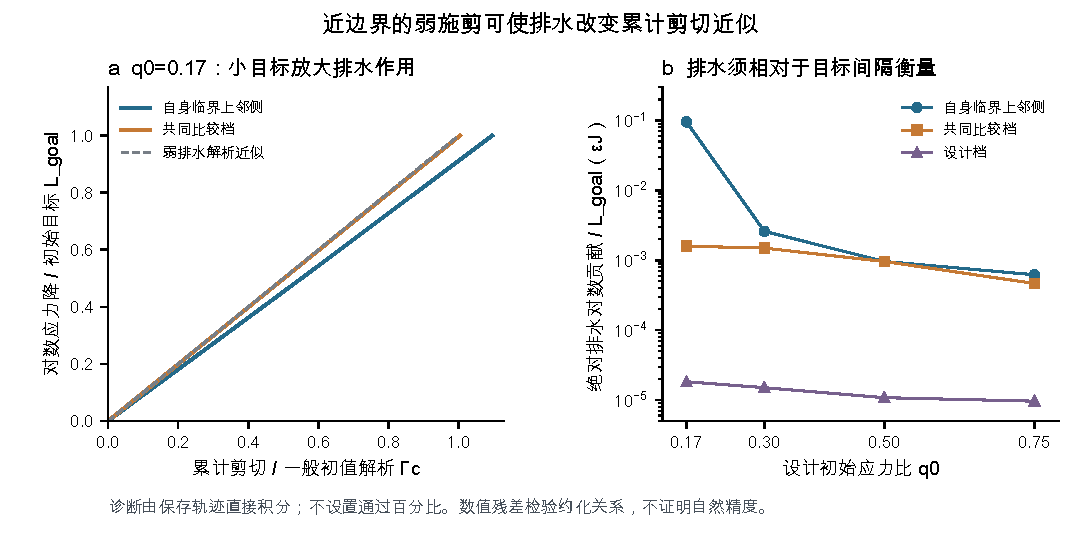
\includegraphics[width=152mm,trim=0 24 0 20,clip]{figures/q2/fig08_initial_state_diagnostics.pdf}
\caption{近边界初态的排水诊断。左图对比略高于临界剪切系数的弱施剪档与共同$\chi_{\rm cmp}$档的应力变化；右图为各诊断轨迹的排水绝对贡献与目标间隔之比。}\label{fig:q2diag}
\end{figure}
\FloatBarrier

\noindent\hspace*{2em}\topic{材料、时间窗与压力形状的影响}

固定$H_0=1$ m、$q_0=0.50$，分别取$m_0=0.54$和0.57；与$m_{\rm crit}=0.60$相比，改为0.59时临界根分别增加20.1\%和50.8\%。$m_{\rm crit}=0.54$时初始有效应力上升。对$m_0=0.54$、$H_0=1$ m、$q_0=0.50$，在相对27 s起始的33、53、73 s窗口分别求根，$\chi^*I_U$依次为0.98124、0.98084和0.98074。

压力剖面的指数$n$控制超孔压随厚度方向衰减的形状。改变该形状时，平均应力、顶面排水与零接触应力层条件须相应改变。对未分层形状$p_e=e(1-x^n)$（$n>1$），可得
\[
s=E/2-\frac{n}{n+1}e,\qquad J=\frac{nke}{\mu H},\qquad q_c(n)=\frac{n-1}{2(n+1)}. \tag{17}
\]
对应分层支取$r=\sqrt{(s/E)/q_c(n)}$、$e=E[1-(n-1)r/n]$，下部$p_e=e-Ex^n/(nr^{n-1})$，上部$p_e=E(1-x)$，通量为$kE/(\mu H)$。在$m_0=0.54$、$H_0=1$ m、$q_0=0.50$及73 s速度窗下，$n=2$和$n=3$的起始应力比分别为$1/6$和$1/4$，$n=3$的条件根低36.4\%（图~\ref{fig:q2shape}）。在$n=2$和相同条件下，将速度曲线整体上移或下移1.5 m/s，条件根为$2.21$—$2.32\times10^{-4}$ m$^{-1}$。

\begin{figure}[htbp]
\centering
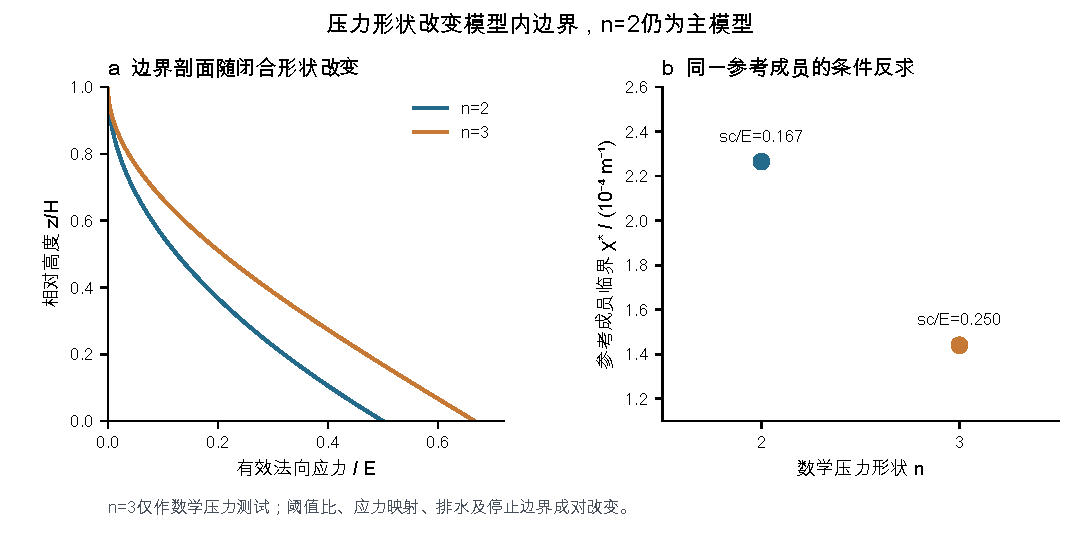
\includegraphics[width=152mm,trim=0 24 0 20,clip]{figures/q2/fig05_closure_sensitivity.pdf}
\caption{不同压力剖面假设下的起始边界比较。两条曲线对应各自的模型内起始边界。}\label{fig:q2shape}
\end{figure}
\FloatBarrier




\FloatBarrier
\subsection{问题三}
\renewcommand{\thefigure}{3-\arabic{figure}}\setcounter{figure}{0}
\renewcommand{\thetable}{3-\arabic{table}}\setcounter{table}{0}
\questionline{第三问：预测局部临界条件的首达时间，分析覆盖率、预警余量与目标到达。}

\subsubsection*{1）模型的准备}

\noindent\hspace*{2em}\topic{预测对象与输入}

问题二给出了局部饱和材料柱的孔压支承层起始边界；问题三在该动力系统上进一步预测何时首次达到边界。记平均有效法向应力比$q=s/E$，二次压力剖面的边界$q_c=1/6$。沿用事件反演速度曲线的选定区间$t_{\rm ref}\in[27,100]$ s，令$t=t_{\rm ref}-27$ s，预测窗为$0\le t\le73$ s；$t=0$为选定计算窗起点，初态在此设置。对初始有效且$q_0>q_c$的材料柱，定义局部首达时间
\[
\tau_L=\inf\{t\in(0,73\,\mathrm{s}]:q(t)\le q_c\}.
\tag{18}
\]
窗内首达输出有限$\tau_L$；完整有效计算窗内未达到边界时记为独立的“窗内未达”类别$\bot$。

参考速度为该事件的事后反演读图曲线。对整条曲线的每个速度节点加入同一偏移$d$，逐节点截零后再分段线性插值。记$t_i=t_{\rm ref,i}-27$ s，节点$t_i$处参考速度为$U_{\rm ref,i}$、处理后为$U_i$，则
\[
\begin{gathered}
U_i(d)=\max\{0,U_{\rm ref,i}+d\},\qquad
U(t;d)=(1-\lambda_i)U_i(d)+\lambda_i U_{i+1}(d),\\
\lambda_i=(t-t_i)/(t_{i+1}-t_i),\qquad d\in[-a,a],\quad a=1.5\ \mathrm{m/s}.
\end{gathered}
\tag{19}
\]
剪切率沿用问题二的$\dot\gamma=\chi U$，单位为s$^{-1}$。主要概率分析固定初态$q_0=0.50$，选用强施剪$\chi=0.02$ m$^{-1}$和近临界$\chi=2.265378784906\times10^{-4}$ m$^{-1}$两种设计条件；$d$分别采用对称三角分布$\mathrm{Tri}(-a,0,a)$、均匀分布$\mathrm{U}(-a,a)$和低速偏向三角分布$\mathrm{Tri}(-a,-a,a)$，其中三角分布三个参数依次为下界、众数和上界。

\subsubsection*{2）模型的建立}

\noindent\hspace*{2em}\topic{分段映射与稳健预测集合}

固定初态、材料和施剪条件后，材料柱方程将速度偏移$d$映射为有限首达时间或窗内状态。对第$r$种偏移分布$F_r$，首达子累积分布$H_r(t)$给出全体情景中至时刻$t$已首达的质量：
\[
H_r(t)=\int\mathbf1\{\text{窗内首达},\ \tau_L(d)\le t\}\,\mathrm dF_r(d).
\tag{20}
\]
对输入域的类别分界和有限首达段进行自适应细分，有限段用形状保持分段三次插值（PCHIP）\cite{q3pchip}，再在每个输入段反解$\tau_L(d)\le t$得到偏移区间$[\ell_j,u_j]$，按$F_r(u_j)-F_r(\ell_j)$计算该段质量并对各段求和。窗末的$H_r(73\,\mathrm{s})$为窗内首达质量，未达质量单独保留。

令$I=[L,U]$为窗内有限时间区间，$\eta\in\{0,1\}$表示预测集合是否包含未达类别；$p_{\bot,r}$为第$r$种分布的窗内未达质量。对声明的三种分布同时要求集合质量不低于$1-\alpha_{\rm cov}=0.95$，在共同固定时间网格上选择有限宽度最短的集合：
\[
\min_{I,\eta}(U-L),\quad
\text{s.t.}\quad\min_r\{H_r(U)-H_r(L^-)+\eta p_{\bot,r}\}\ge1-\alpha_{\rm cov}.
\tag{21}
\]
其中$H_r(L^-)$使闭区间左端点计入，$\alpha_{\rm cov}=0.05$为目标漏覆盖率。三种输入分布共享同一确定性响应映射，改变的是概率权重。名义分布为对称三角分布：名义中央集合按2.5\%与97.5\%累计质量定位端点，高分位超出有限首达质量时附加窗内未达；名义最短集合在该分布下选择有限宽度最短的集合；稳健最短集合同时满足三种分布的质量要求。

\subsubsection*{3）模型的求解与分析}

\noindent\hspace*{2em}\topic{时间预测与模拟覆盖}

强施剪的稳健95\%有限预测区间为\important{[0.775, 0.815] s}；近临界预测集合由有限区间\important{[71.40, 72.95] s}与73 s内未达类别组成（表~\ref{tab:q3set}，图~\ref{fig:q3sets}）。时间均相对选定计算窗起点。连续积分得到的最差分布质量分别为0.975799和0.964297。

\begin{table}[htbp]
\centering
\caption{两种施剪条件下的稳健95\%首达预测集合}\label{tab:q3set}
\fontsize{9.5}{12}\selectfont
\setlength{\tabcolsep}{5pt}
\begin{tabularx}{\textwidth}{X c c c}
\toprule
条件 & 窗内时间区间/s & 窗内未达 & 最差族积分质量 \\
\midrule
强施剪 & [0.775, 0.815] & 不含 & 0.975799 \\
近临界 & [71.40, 72.95] & 包含 & 0.964297 \\
\bottomrule
\end{tabularx}
\end{table}

\begin{figure}[htbp]
\centering
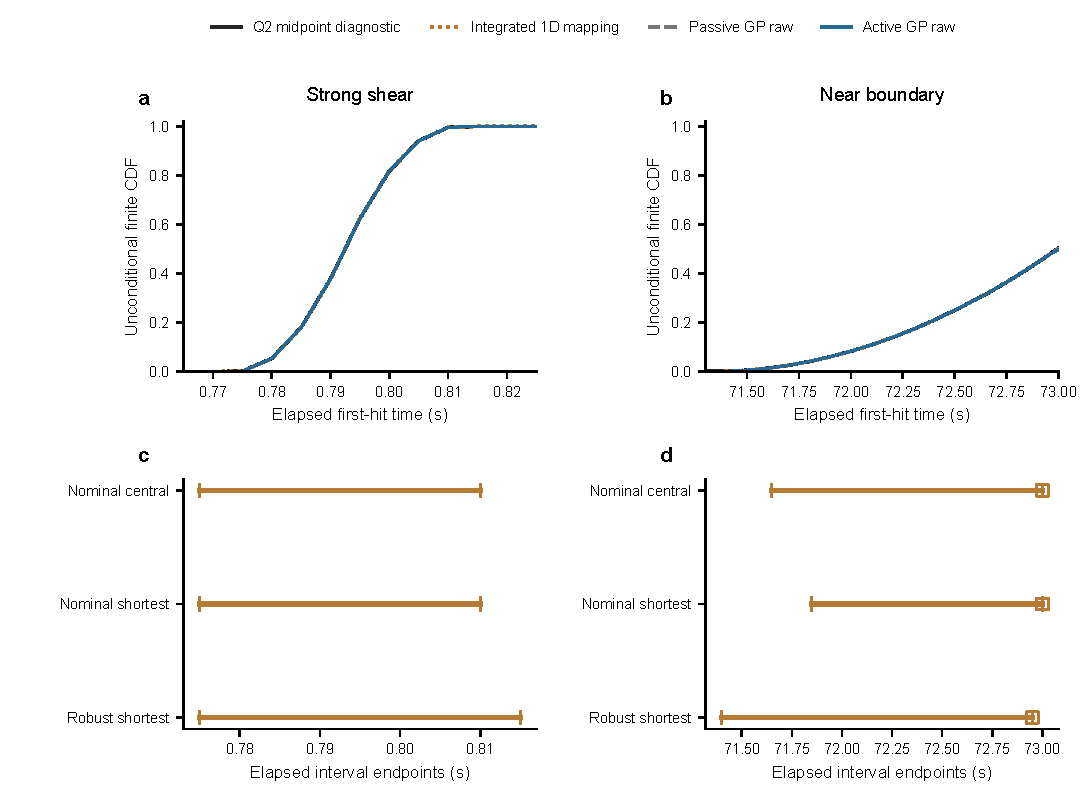
\includegraphics[width=0.95\textwidth,trim=0 0 0 210,clip]{figures/q3/fig04_probability_sets.pdf}
\caption{强施剪（c）与近临界（d）的首达预测集合。每栏从上至下为名义中央、名义最短和三分布稳健最短集合；空心方框表示附加窗内未达类别，横轴为自选定计算窗起点计的有限区间端点。}\label{fig:q3sets}
\end{figure}
\FloatBarrier

为检验上述两套集合在声明分布下的模型模拟包含率，分别从两种施剪条件和三种偏移分布生成随机成员，每项4096个，共24576个。目标漏覆盖率为$\alpha_{\rm cov}=0.05$；六项声明的总体模拟错误预算取$\delta_{\rm sim}=0.05$，每项分配$\delta_{\rm sim}/6$。对包含数$k$和样本数$n$，以单侧Clopper--Pearson精确二项下界\cite{q3cp}$\ell=B^{-1}(\delta_{\rm sim}/6;k,n-k+1)$评价包含概率，其中$B^{-1}$为对应Beta分布分位数。六项模拟包含比例和同时保护下界见表~\ref{tab:q3coverage}；强施剪和近临界的最低下界分别为0.970003和0.956011，均高于0.95。

\begin{table}[htbp]
\centering
\caption{两种施剪条件、三种速度偏移分布下的模拟包含率}\label{tab:q3coverage}
\fontsize{9.5}{12}\selectfont
\setlength{\tabcolsep}{4pt}
\begin{tabularx}{\textwidth}{X X c c c}
\toprule
条件 & 分布 & 包含数/4096 & 包含比例 & 精确单侧下界 \\
\midrule
强施剪 & 对称三角 & 4090 & 0.998535 & 0.996376 \\
强施剪 & 均匀 & 3999 & 0.976318 & 0.970003 \\
强施剪 & 低速偏向三角 & 4094 & 0.999512 & 0.997893 \\
近临界 & 对称三角 & 3979 & 0.971436 & 0.964584 \\
近临界 & 均匀 & 3947 & 0.963623 & 0.956011 \\
近临界 & 低速偏向三角 & 4047 & 0.988037 & 0.983319 \\
\bottomrule
\end{tabularx}
\end{table}

\noindent\hspace*{2em}\topic{初态与临界响应}

19个初始应力比与17个速度偏移组成323个设计点，两种施剪条件共646个情景：强施剪323个窗内首达，近临界179个首达、144个窗内未达（图~\ref{fig:q3phase}）。近临界且$d=0$时，$q_0=0.30$与0.50的首达时间分别为41.682 s和72.997 s，$q_0=0.75$为窗内未达；在$q_0=0.50$、$d=0$下，将近临界$\chi$降低1\%得到窗内未达，提高1\%得到72.331 s首达。

\begin{figure}[htbp]
\centering
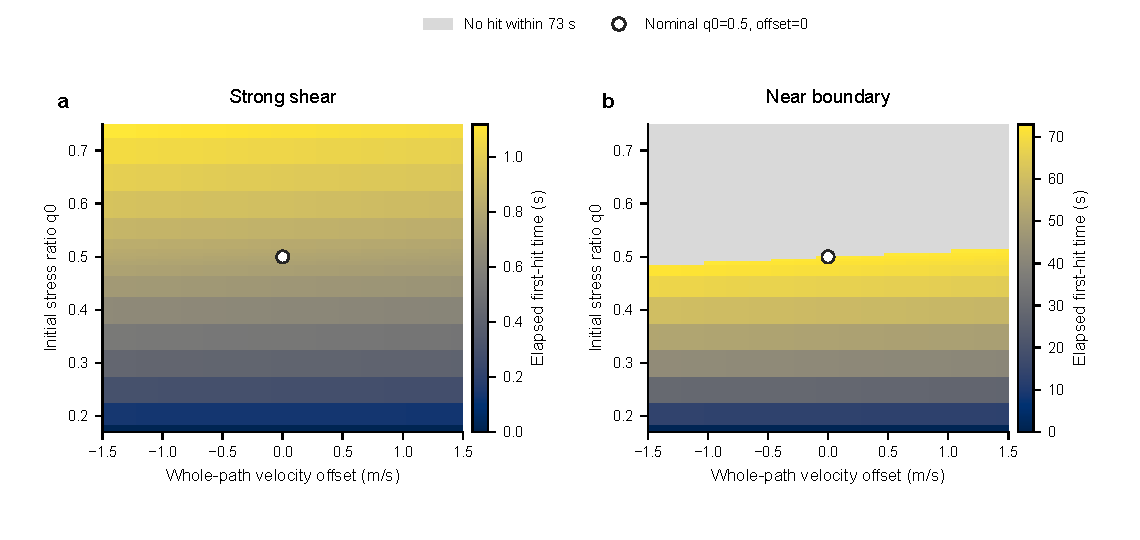
\includegraphics[width=0.95\textwidth]{figures/q3/fig07_initial_velocity_sensitivity.pdf}
\caption{初始应力比与整条速度偏移对应的首达响应。左栏为强施剪、右栏为近临界；横轴$d$为整条速度偏移（m/s），纵轴$q_0$为初始应力比，两栏色标范围不同，均表示自选定窗起点计的有限首达时间（s）；灰色为73 s内未达，白圈为$q_0=0.50$、$d=0$。}\label{fig:q3phase}
\end{figure}
\FloatBarrier

在首达处横截且$\dot q(\tau_L)\ne0$时，相同局部状态增量$\delta q$对应的一阶时间变化为
\[
\delta\tau_L\simeq-\frac{\delta q}{\dot q(\tau_L)}.
\tag{22}
\]
取$\delta q=0.001$，强施剪与近临界的时间响应分别为0.00428 s和0.35857 s，后者约为前者的83.8倍。该比较说明慢横截对局部状态裕量的报时放大；近临界名义首达距窗末约0.002905 s，扰动可使结果在首达与未达之间切换。三种偏移分布下，近临界窗内未达质量依次为0.4983、0.4991和0.7491。

\noindent\hspace*{2em}\topic{发布、行动与局部预警余量}

设$d_{\rm pub}$为自选定窗起点至发布的延迟，$d_{\rm act}$为发布后的行动历时，则局部首达相对行动就绪时刻的余量为
\[
L_L=\tau_L-d_{\rm pub}-d_{\rm act}.
\tag{23}
\]
$L_L>0$表示行动就绪后尚有时间，$L_L<0$表示就绪晚于局部首达。强施剪下发布延迟1 s、行动历时0 s，对应有限余量[−0.225, −0.185] s；近临界下发布延迟1 s、行动历时15 s，对应[55.40, 56.95] s，另保留窗内未达类别。图~\ref{fig:q3lead}给出不同延迟下的变化，强施剪的负余量提示预警启动需要前置。

\begin{figure}[htbp]
\centering
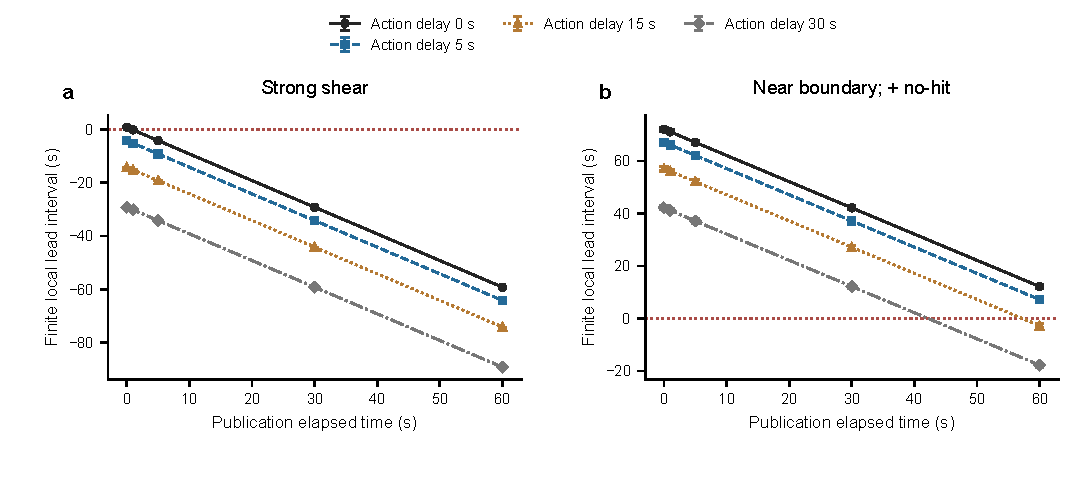
\includegraphics[width=0.95\textwidth]{figures/q3/fig05_local_lead.pdf}
\caption{不同发布延迟和行动历时下的局部有限余量。左栏为强施剪、右栏为近临界；横轴为发布延迟（s），四条线对应行动历时0、5、15、30 s，纵轴为有限余量（s）。零线区分行动就绪早于或晚于局部首达；近临界集合保留窗内未达类别。}\label{fig:q3lead}
\end{figure}
\FloatBarrier

\noindent\hspace*{2em}\topic{理想常坡目标到达}

为计算空间目标的条件余量，设传播入口相对时刻$T_{\rm in}$与局部首达时刻$T_L=\tau_L$相同；目标旅行时长为$\Delta T_A$，到达时刻与行动余量分别为
\[
T_A=T_{\rm in}+\Delta T_A,\qquad L_A=T_A-d_{\rm pub}-d_{\rm act}.
\tag{24}
\]
在8°理想常坡、恒定法向层厚2 m的算例中，以沿坡距入口1000 m处为固定测试断面，自传播入口起算的传播时间窗取180 s。采用Voellmy摩擦参数$\mu_V$（无量纲）和湍阻参数$\xi$（m/s²）构造五个固定参数情景；$\mu_V$与问题二的悬液黏度$\mu$分别定义。记$z$为自入口起算的传播时间、$x$为沿坡位移、$v$为速度，$\vartheta=8^\circ$、恒定法向层厚$H_A=2$ m、$g=9.81$ m/s²，则单方向标量运动关系和初始条件为
\[
\frac{\mathrm dx}{\mathrm dz}=v,\qquad
\frac{\mathrm dv}{\mathrm dz}=g(\sin\vartheta-\mu_V\cos\vartheta)-\frac{gv^2}{\xi H_A},\qquad x(0)=v(0)=0.
\tag{25}
\]
由解析位移关系解$x(z)=1000$ m得到旅行时长；五个情景中三例到达目标，两例在180 s内未到（表~\ref{tab:q3target}）。将各情景旅行时间与对应局部首达集合相加，即得目标到达时间与行动余量；图~\ref{fig:q3target}展示发布延迟60 s、行动历时30 s时的有限余量。

\begin{table}[htbp]
\centering
\caption{8°理想常坡至1000 m测试断面的五个传播情景}\label{tab:q3target}
\fontsize{9.5}{12}\selectfont
\setlength{\tabcolsep}{4pt}
\begin{tabularx}{\textwidth}{c c c X}
\toprule
情景 & $\mu_V$ & $\xi$/(m/s²) & 旅行时长或传播窗状态 \\
\midrule
S1 & 0.03 & 200 & 155.395 s \\
S2 & 0.03 & 2000 & 61.260 s \\
S3 & 0.13 & 200 & 180 s内未到 \\
S4 & 0.13 & 2000 & 180 s内未到 \\
S5 & 0.09 & 399.052 & 167.147 s \\
\bottomrule
\end{tabularx}
\end{table}

\begin{figure}[htbp]
\centering
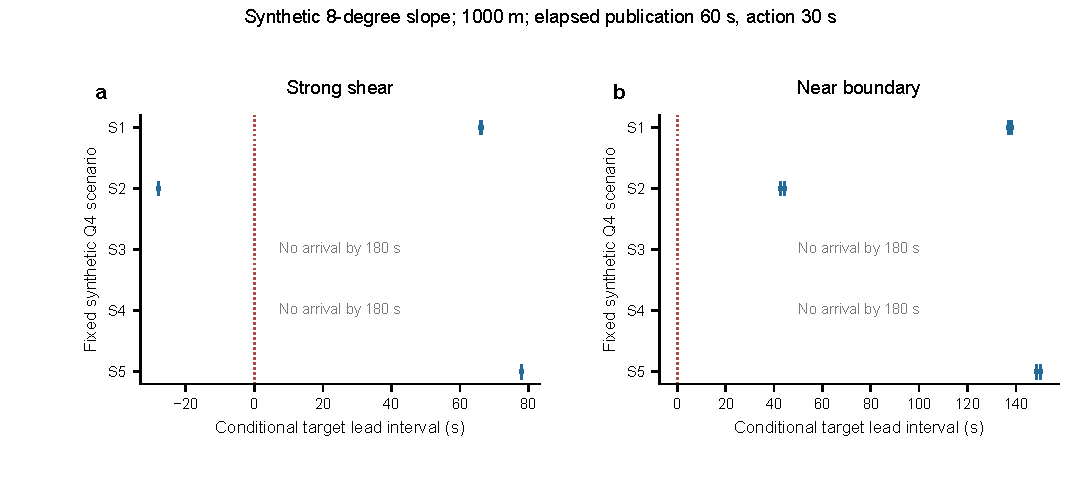
\includegraphics[width=0.95\textwidth]{figures/q3/fig06_synthetic_target_lead.pdf}
\caption{理想常坡固定1000 m目标的条件行动余量。左栏为强施剪、右栏为近临界；横轴为目标行动余量（s），纵轴S1—S5为表~\ref{tab:q3target}的参数情景。发布延迟60 s、行动历时30 s；S3、S4在180 s传播窗内未到，虚线表示零余量。}\label{fig:q3target}
\end{figure}
\FloatBarrier


\FloatBarrier
\subsection{问题四}
\renewcommand{\thefigure}{4-\arabic{figure}}\setcounter{figure}{0}
\renewcommand{\thetable}{4-\arabic{table}}\setcounter{table}{0}
\questionline{第四问：建立规定入口后的二维传播仿真，分析到达、覆盖及关键参数。}

\subsubsection*{1）模型的准备}

\noindent\hspace*{2em}\topic{计算区域与入口条件}

本问以已形成的等效流体进入指定断面为传播起点，入口开始时刻记为相对0 s。局部目标断面和口岸目标断面距入口的参考轴线长度分别约2.119 km和14.188 km。问题三的材料柱首达与本问的规定入口分别定义，两者采用各自的时间原点。计算在水平坐标下进行，流深为竖直厚度；地形采用投影至UTM 45N（EPSG:32645）的Copernicus GLO-30及ASTER GDEM V003\cite{q4data1,q4data2}，各产品独立形成15 m插值支持，再采样到不同计算网格；15 m支持为插值表达。

规定入口宽30 m、向西速度30 m/s，初始域为干床；入口脉冲结束后关闭，规定的下游区段允许出流。入口流量采用总体积$V$、历时$T$确定的对称三角脉冲，峰值为$2V/T$。基准设定$V=8\times10^5$ m³、$T=960$ s；双峰情景由两个相邻的半体积、半历时对称三角脉冲组成。目标断面上的最大竖直流深首次达到0.1 m时记为到达，首达时刻保留计算步构成的括区。局部域分析采用1800 s计算窗，完整河段采用3600 s计算窗。

\subsubsection*{2）模型的建立}

\noindent\hspace*{2em}\topic{固定床二维守恒浅流}

设$h$为竖直流深（m），$\mathbf u$为深度平均水平速度（m/s），$z$为固定床高（m），$g=9.81$ m/s²；$\mu_V$为Voellmy摩擦系数，$\xi$为湍阻参数。固定床、常密度条件下，以质量和动量守恒描述流动\cite{q4shallow}：
\[
\frac{\partial h}{\partial t}+\nabla\!\cdot(h\mathbf u)=0,
\tag{26}
\]
\[
\frac{\partial(h\mathbf u)}{\partial t}+
\nabla\!\cdot\left(h\mathbf u\otimes\mathbf u+\tfrac12gh^2\mathbf I\right)
=-gh\nabla z-\mu_Vgh\frac{\mathbf u}{|\mathbf u|}
-\frac{g}{\xi}|\mathbf u|\mathbf u.
\tag{27}
\]
其中$\mathbf I$为单位张量，$\otimes$为张量积；$\mu_V$无量纲，$\xi$的单位为m/s²。零速度处摩擦按停止条件处理。空间上采用有限体积HLL通量、受限重构和静水重构\cite{q4hydro}，时间推进结合非反向隐式摩阻更新。入口流量以时间步上的解析积分分配；按边界通量核对体积收支，并记录有效到达和有效计算窗内未达。

\noindent\hspace*{2em}\topic{参数筛选与多保真代理}

以局部断面的最大深度余量$h_{\max}-0.1\,\mathrm m$为筛选响应，以归一化参数步长0.6计算基本效应，其八条轨迹的绝对值均值记为$\mu^*$（m），在$V\in[2,8]\times10^5$ m³、$T\in[720,1200]$ s、$\mu_V\in[0.03,0.15]$、$\xi\in[250,1000]$ m/s²内进行Morris分析。Morris计算采用40 m网格和1800 s窗；八条完整轨迹共有40个节点、38个不同查询；$V$、$T$及$\xi$在对数尺度构造轨迹。再固定$T=960$ s、$\xi=500$ m/s²，在$(\log V,\mu_V)$切片上比较代理的到达边界。

取同一连续地形支持上的40 m和30 m网格为低、高分辨率层。高斯过程（GP）代理采用Matérn 5/2核，以无量纲响应$y$表示最大断面流深：
\[
y=\log\!\left(\frac{h_{\max}+0.1\,\mathrm m}{0.2\,\mathrm m}\right),
\qquad y=0\ \Longleftrightarrow\ h_{\max}=0.1\,\mathrm m.
\tag{28}
\]
多保真代理以高层响应$f_H=\rho f_L+e$连接低层$f_L$与层间差异$e$；$\rho$为层间系数，$f_L$和$e$的先验相互独立，$\rho$和核参数由训练集最大似然拟合；主动策略按边界附近高层预测方差的预期下降及物理调用成本选择新点\cite{q4mf}。比较四组：A为16个高层点的单层被动代理；B为16个高层和24个低层点的被动多保真代理；Bm与C均为16个高层、32个低层点，分别采用被动和主动选点；C从共同8个高层与24个低层初始点出发，再主动增加8个高层及8个低层点。

\subsubsection*{3）模型的求解与分析}

\noindent\hspace*{2em}\topic{局部传播与关键因素}

在$\mu_V=0.05$、$\xi=500$ m/s²的基准入口及30 m网格下，局部目标0.1 m首达括区为\important{[731.535, 731.808] s}，断面最大流深为10.020 m（图~\ref{fig:q4depth}）。入口速度由30降至24 m/s，或入口宽度由30增至40 m时，首达括区上界分别为733.868 s和733.380 s，显示这两个指定扰动下局部结果的变化。

\begin{figure}[htbp]
\centering
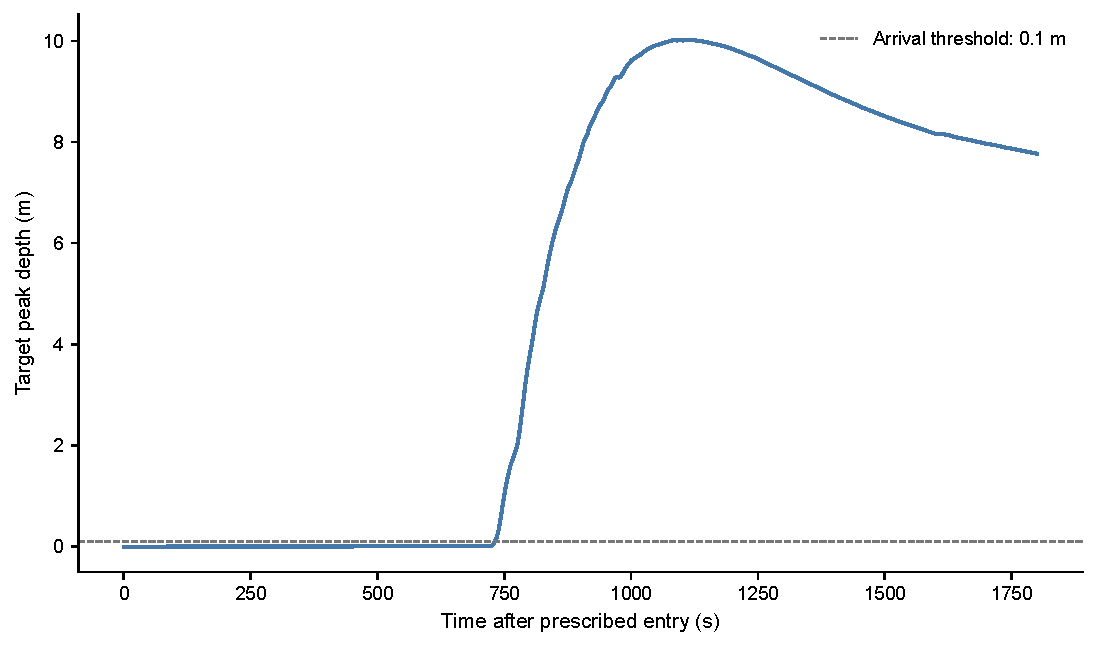
\includegraphics[width=0.90\textwidth]{figures/q4/02_target_depth.pdf}
\caption{局部基准断面流深过程。横轴为自规定入口开始计的相对时间，纵轴为断面瞬时最大竖直流深，虚线为0.1 m到达阈值。}\label{fig:q4depth}
\end{figure}
\FloatBarrier

Morris八条轨迹中有14个不同查询到达、24个在计算窗内未达。$\mu^*$按$\mu_V$、$V$、$T$、$\xi$依次为7.176、2.489、0.819、0.602 m，表明在所设范围和断面深度余量响应下，摩擦系数与入口体积的影响较大。

\noindent\hspace*{2em}\topic{完整河段覆盖}

对Copernicus 30 m、Copernicus 40 m、ASTER 40 m及Copernicus 40 m双峰四个情景，口岸目标断面均在3600 s窗内未达到0.1 m，且窗末保持流体运动。四组均采用上述基准总体积、历时、入口宽度、速度和摩阻参数；双峰情景采用双峰入流过程。表~\ref{tab:q4full}分别列出计算窗内曾达到0.1 m的覆盖面积与窗末瞬时覆盖面积；图~\ref{fig:q4footprint}给出Copernicus 40 m单峰情景的空间分布。

\begin{table}[htbp]
\centering
\caption{完整河段四个条件情景的3600 s窗内结果}\label{tab:q4full}
\fontsize{9.5}{12}\selectfont
\setlength{\tabcolsep}{4pt}
\begin{tabularx}{\textwidth}{X c c c}
\toprule
地形与网格 & 域内最大流深/m & 曾过阈面积/m² & 窗末面积/m² \\
\midrule
Copernicus 30 m & 22.180 & 301500 & 201600 \\
Copernicus 40 m & 23.571 & 313600 & 212800 \\
ASTER 40 m & 29.089 & 145600 & 102400 \\
Copernicus 40 m双峰 & 23.686 & 313600 & 212800 \\
\bottomrule
\end{tabularx}
\end{table}

\begin{figure}[htbp]
\centering
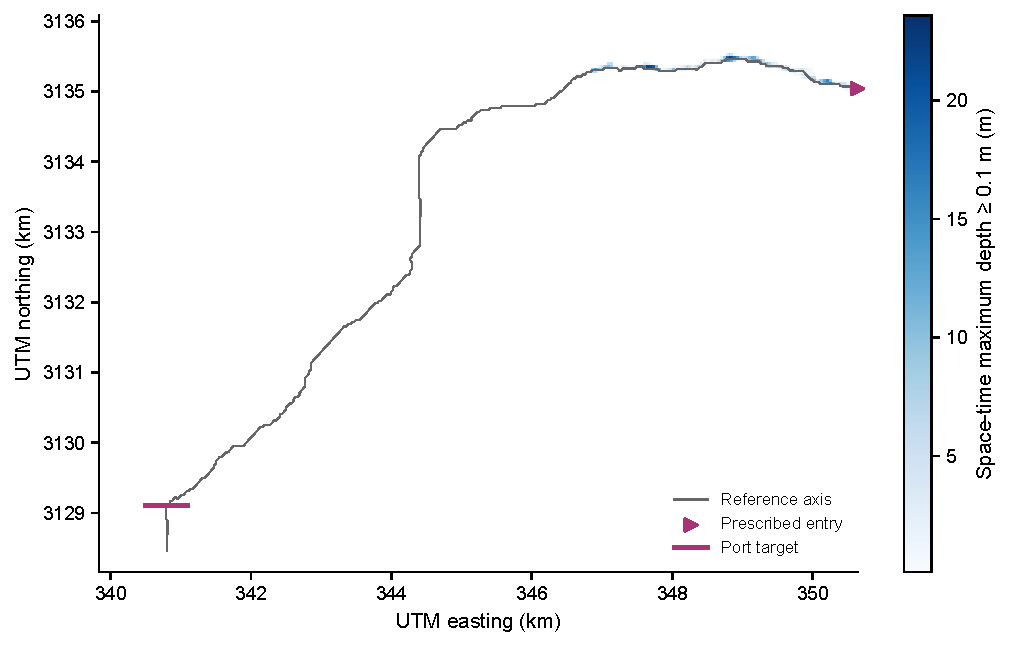
\includegraphics[width=0.90\textwidth]{figures/q4/07_full_footprint.pdf}
\caption{Copernicus 40 m完整河段情景的窗内覆盖。色值表示3600 s内曾达到0.1 m单元的最大竖直流深；灰线为参考轴线，三角标记为规定入口，短线为口岸目标断面；横、纵轴为UTM东、北坐标（km）。}\label{fig:q4footprint}
\end{figure}
\FloatBarrier

\noindent\hspace*{2em}\topic{四策略到达边界判断}

采用种子137的64个不同训练查询（40个低层、24个高层）；测试采用16个全域点和8个开发预测边界点，预测完成后再取得相同坐标的高、低层结果。全域16点中有4个高层模拟到达，四策略均识别这4点；边界带8点全部在窗内未达。各策略的误报数和全域均方根误差（RMSE）见表~\ref{tab:q4gp}。

\begin{table}[htbp]
\centering
\caption{种子137四策略在原24个独立测试坐标上的到达判断与误差}\label{tab:q4gp}
\fontsize{9.5}{12}\selectfont
\setlength{\tabcolsep}{3pt}
\begin{tabularx}{\textwidth}{X c c c c}
\toprule
策略 & 全域误报/16 & 边界误报/8 & 全域$y$ RMSE & 深度余量RMSE/m \\
\midrule
A 单层被动 & 3 & 2 & 0.64657 & 1.55064 \\
B 多保真被动 & 2 & 2 & 0.79706 & 1.73590 \\
Bm 数量匹配被动 & 1 & 0 & 0.30945 & 0.53211 \\
C 多保真主动 & 0 & 0 & 0.30415 & 1.64786 \\
\bottomrule
\end{tabularx}
\end{table}

原24点对照中，C的到达类别全部正确；预测边界带没有高层模拟到达成员，故该带漏达率为不适用。全域原始深度余量RMSE中，Bm为0.53211 m、C为1.64786 m，反映到达类别和深度幅值是两个不同评价对象。四组采用同一固定历时和湍阻参数切片。
\FloatBarrier

\Needspace{8\baselineskip}
\noindent\hspace*{2em}\topic{临界摩擦区间与端点检验}

为检验到达边界，在固定$T=960$ s、$\xi=500$ m/s²及局部30 m网格、1800 s窗下，分别取$V_1=336358.566$ m³和$V_2=672717.132$ m³。两条体积切片共完成14次高层模拟查询，所得到达与未达之间的摩擦系数括区依次为\important{[0.06000, 0.06375]}和\important{[0.07875, 0.08250]}。每条切片的两个端点分别为到达和窗内未达；对四端点评价种子137对应的四组代理，结果见表~\ref{tab:q4critical}。这些端点由临界搜索选出，展示的是指定模型和时窗下的边界判断。

\begin{table}[htbp]
\centering
\caption{四策略在两条体积切片的四个高层模拟端点上的表现}\label{tab:q4critical}
\fontsize{9.5}{12}\selectfont
\setlength{\tabcolsep}{3pt}
\begin{tabularx}{\textwidth}{>{\centering\arraybackslash}X c c c c c}
\toprule
策略 & TP/FN/FP/TN & $y$ RMSE & 深度余量RMSE/m & $V_1$根距 & $V_2$根距 \\
\midrule
A & 2/0/2/0 & 1.77867 & 0.95205 & 0.01286 & 0.01746 \\
B & 2/0/2/0 & 2.10412 & 1.79631 & 0.00937 & 0.03562 \\
Bm & 2/0/1/1 & 1.09126 & 0.45808 & 0.00861 & 0 \\
C & 2/0/2/0 & 0.89954 & 0.27562 & 0.00378 & 0.00182 \\
\bottomrule
\end{tabularx}
\end{table}

表中TP、FN、FP、TN依次为正确到达、漏达、误报和正确未达的点数；根距为各代理预测摩擦临界根到对应高层模拟括区的距离，根在括区内时为零。主动组C在四端点误报2个，其$y$响应RMSE为0.89954；Bm误报1个，$V_2$预测根落在括区内。分类、连续响应和根定位分别评价。种子271的四组模型对既有24点作描述性回放，A、B、Bm、C的误报数依次为2、2、2、0，均无漏达。

\noindent\hspace*{2em}\topic{物理核验与状态发布}

将GP结果作为预估，以同配置30 m传播计算核定到达状态；核对输入、网格与参数、时窗、目标阈值及质量和动量收支后，发布有效“到达”或“1800 s窗内未达”结果。相同配置的有效物理结果可复用。对$V=475682.846$ m³的两个新增参数点，$\mu_V=0.0675$时目标到达、峰深1.743419 m，首达括区为[1467.34219, 1467.62929] s；$\mu_V=0.075$时1800 s内未达。两次新增传播计算的子进程墙时之和为67.30125 s。四个历史端点与两个新增点的发布结果均与各自有效物理证据一致；原GP对这六条记录预估时产生3个误报，该比较反映核验接口的一致性。

\FloatBarrier


\section{模型评价、改进与推广}

\subsection{模型的优点}

问题一以年度等权多窗口比较描述环境特征，兼顾因素排序与联合结构。问题二以守恒与剪胀关系连接受剪、排水和孔压；问题三同时保留首达时间与窗内未达类别。问题四将地形、规定入流与守恒浅流结合，并以物理核验支撑到达状态发布。

\subsection{模型的缺点}

历史参考年份有限，因素位置随窗口和参考配置变化。材料柱采用局部平均状态及理想化压力剖面；局部首达与已形成流入口的实测对应尚待建立。传播结果依赖固定床、地形和设计入流；临界代理出现误报，物理核验增加计算费用。

\subsection{模型的改进与推广}

可补充多年份、多站点观测，扩展历史比较；通过材料试验与现场观测校核初态、渗透率和压力剖面。进一步建立局部触发至入口的状态和时钟对应，并结合实测河床、断面流量与多时空资料校核传播，在其他沟谷按地形与入口条件重新设置参数。

\FloatBarrier
\stepcounter{section}
\renewcommand{\refname}{\chinese{section}、\quad 参考文献}
\Needspace{8\baselineskip}
\begin{thebibliography}{99}
\small
\raggedright
\bibitem{ref1} 2026年第七届MathorCup数学应用挑战赛——大数据竞赛组委会. 赛道B：泥石流灾害预报及防灾策略[Z]. 2026年初赛题面，2026.
\bibitem{ref2} 马耀明，马伟强，谢志鹏，王宾宾，陈学龙，韩存博，西藏吉隆高寒山区地气相互作用逐小时综合观测数据集（2021—2026），国家青藏高原科学数据中心，\url{https://doi.org/10.11888/Atmos.tpdc.303600}，访问日期2026-10-24。
\bibitem{era5api} Open-Meteo，Historical Weather API: models, hourly variables, time zones and grid-cell selection，\url{https://open-meteo.com/en/docs/historical-weather-api}，访问日期2026-10-30。
\bibitem{ref3} Wang B, Ma Y, Hu Z, et al. Quantifying the spatial-seasonal patterns of land–atmosphere water, heat and CO2 flux exchange over the Tibetan Plateau from an observational perspective，Earth System Science Data，18：1147–1164，2026. \url{https://doi.org/10.5194/essd-18-1147-2026}.
\bibitem{ref7} Jackson J E, Mudholkar G S. Control Procedures for Residuals Associated With Principal Component Analysis，Technometrics，21(3)：341–349，1979. \url{https://doi.org/10.1080/00401706.1979.10489779}.
\bibitem{q2yin} 殷跃平，张仕林，高少华，等. 尼泊尔蓝塘里壤峰“8·26”冰岩崩致吉隆泥石流灾难研究[Z]. 录用稿, 2026. \url{https://doi.org/10.16031/j.cghc.202610008}.
\bibitem{q2kang} Kang J, Lucas A, Mangeney A, et al. Frictional weakening in the highly mobile 2025 Blatten rock and ice avalanche in Switzerland，Communications Earth \& Environment，7：722，2026. \url{https://doi.org/10.1038/s43247-026-03983-1}.
\bibitem{q2data} Kang J, Lucas A, Mangeney A, et al.，Dataset for paper “Frictional weakening in the highly mobile 2025 Blatten rock and ice avalanche in Switzerland”，Zenodo，\url{https://doi.org/10.5281/zenodo.21511788}，访问日期2026-10-30。
\bibitem{q2iverson14} Iverson R M, George D L. A depth-averaged debris-flow model that includes the effects of evolving dilatancy. I. Physical basis，Proceedings of the Royal Society A，470(2170)：20130819，2014. \url{https://doi.org/10.1098/rspa.2013.0819}.

\bibitem{q3pchip} Fritsch F N, Butland J. A method for constructing local monotone piecewise cubic interpolants，SIAM Journal on Scientific and Statistical Computing，5(2)：300–304，1984. \url{https://doi.org/10.1137/0905021}.
\bibitem{q3cp} Clopper C J, Pearson E S. The use of confidence or fiducial limits illustrated in the case of the binomial，Biometrika，26(4)：404–413，1934. \url{https://doi.org/10.1093/biomet/26.4.404}.
\bibitem{q4data1} Copernicus，Copernicus WorldDEM-30 / GLO-30，\url{https://dataspace.copernicus.eu/explore-data/data-collections/copernicus-contributing-missions/collections-description/COP-DEM}，访问日期2026-10-30。
\bibitem{q4data2} NASA and METI，ASTER Global Digital Elevation Model V003，NOAA InPort，\url{https://www.fisheries.noaa.gov/inport/item/59575/full-list}，访问日期2026-10-30。
\bibitem{q4shallow} Langham J, Woodhouse M J, Hogg A J, et al.，Simulating shallow morphodynamic flows on evolving topographies，\url{https://doi.org/10.48550/arXiv.2306.16185}，访问日期2026-10-30。
\bibitem{q4hydro} Delestre O, Cordier S, Darboux F, James F. A limitation of the hydrostatic reconstruction technique for Shallow Water equations，Comptes Rendus Mathématique，350：677–681，2012. \url{https://doi.org/10.1016/j.crma.2012.08.004}.
\bibitem{q4mf} Renganathan S A, Rao V, Navon I M. CAMERA: A method for cost-aware, adaptive, multifidelity, efficient reliability analysis，Journal of Computational Physics，472：111698，2023. \url{https://doi.org/10.1016/j.jcp.2022.111698}.
\bibitem{ai_zcode} ZCode，GLM-5.3-Flash，智谱 Z.ai，2026-10-27至2026-10-30。
\bibitem{ai_deepseek} DeepSeek，DeepSeek-V4.1-Flash-1017，深度求索，2026-10-25至2026-10-30。
\end{thebibliography}

\noindent\textbf{AI工具使用声明：}使用的人工智能工具与日期见文献\cite{ai_zcode,ai_deepseek}。

\FloatBarrier
\clearpage
\section{附录}
\subsection*{附录1：单侧假说与多尺度结果}

为检查特定方向的历史位置，另列热力、浅土水分及ERA5格点降水的偏高单侧对照（表~\ref{tab:A1}）。单侧比较采用$\max_w q$，目标与历史端点按相同择窗和式（5）校准。图~\ref{fig:5}给出17项候选在各窗的双侧异常及方向。


\renewcommand{\thefigure}{A\arabic{figure}}\setcounter{figure}{0}
\renewcommand{\thetable}{A\arabic{table}}
\setcounter{table}{0}
\begin{table}[htbp]
\centering
\caption{偏高方向对照的历史校准位置}\label{tab:A1}
\fontsize{9.5}{12}\selectfont
\setlength{\tabcolsep}{4pt}
\begin{tabularx}{\textwidth}{X c c}
\toprule
因素 & 比较方向 & 单侧$S$ \\
\midrule
2 m均温／正温指数 & 偏高 & 0.788 \\
2 m窗口内最大小时均温 & 偏高 & 0.683 \\
24 h块均温变化率 & 偏高 & 0.824 \\
0.1 m含水量 & 偏高 & 0.776 \\
0.1 m土温 & 偏高 & 0.224 \\
ERA5累计总降水 & 偏高 & 0.948 \\
ERA5最大小时总降水量 & 偏高 & 0.948 \\
ERA5有降水小时数 & 偏高 & 0.613 \\
ERA5前期总降水指数 & 偏高 & 0.740 \\
\bottomrule
\end{tabularx}
\end{table}

\begin{figure}[htbp]
\centering
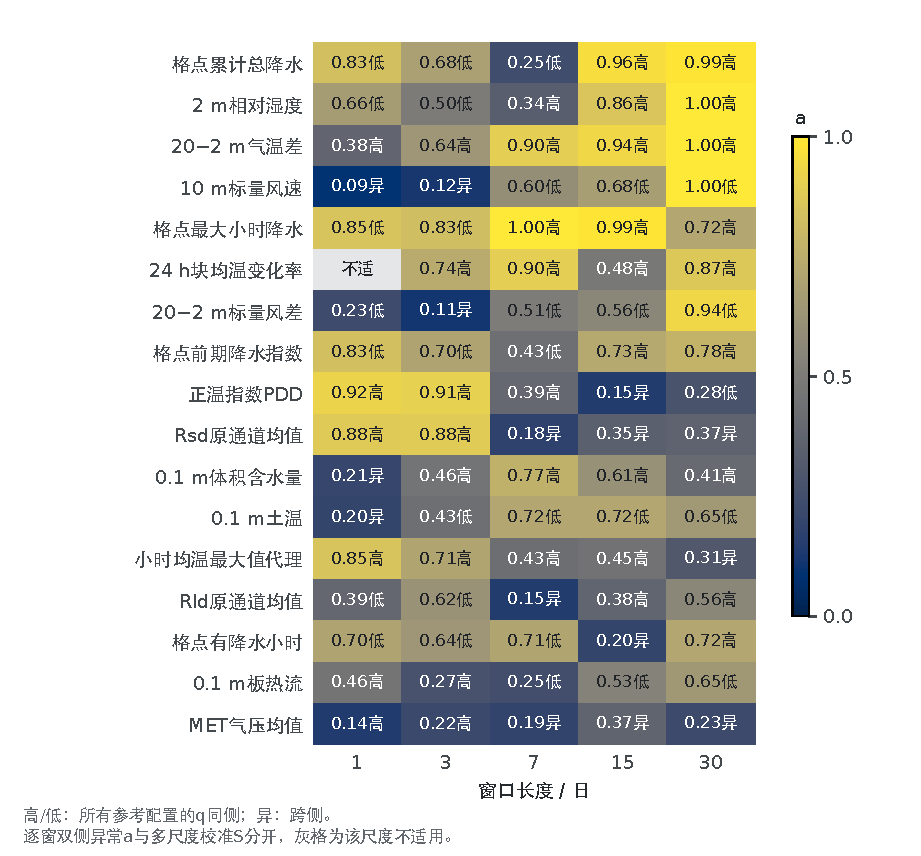
\includegraphics[width=156mm,trim=0 25 0 0,clip]{figures/q1_new/q1_app01_multiscale.pdf}
\caption{17项候选在各固定尺度的异常与方向。颜色和数字为各参考配置平均的单窗双侧异常$a$；“高”“低”表示参考配置方向一致，“异”表示方向分歧，灰色为窗口不适用。}\label{fig:5}
\end{figure}



\FloatBarrier
% 需在导言区加载 \usepackage{fvextra}；继承工程已设置的中西文字体。
\clearpage
\subsection*{附录2：软件与运行命令}
以下列出运行环境及命令，输入路径和输出目录以附件实际内容为准。
\VerbatimInput[breaklines=true,breakanywhere=true,fontsize=\fontsize{8}{10}\selectfont]{appendix_code/software_commands.txt}
\clearpage
\subsection*{附录3：完整程序代码}
以下依次列出数据准备及四问源程序。
\subsubsection*{数据准备}
\noindent\texttt{\detokenize{prepare/clean_all.py}}\par
\VerbatimInput[breaklines=true,breakanywhere=true,fontsize=\fontsize{8}{10}\selectfont]{appendix_code/prepare/clean_all.py}
\noindent\texttt{\detokenize{prepare/clean_data.py}}\par
\VerbatimInput[breaklines=true,breakanywhere=true,fontsize=\fontsize{8}{10}\selectfont]{appendix_code/prepare/clean_data.py}
\noindent\texttt{\detokenize{prepare/era5/download.py}}\par
\VerbatimInput[breaklines=true,breakanywhere=true,fontsize=\fontsize{8}{10}\selectfont]{appendix_code/prepare/era5/download.py}
\noindent\texttt{\detokenize{prepare/netcdf_cleaning.py}}\par
\VerbatimInput[breaklines=true,breakanywhere=true,fontsize=\fontsize{8}{10}\selectfont]{appendix_code/prepare/netcdf_cleaning.py}
\noindent\texttt{\detokenize{prepare/quality_diagnostics.py}}\par
\VerbatimInput[breaklines=true,breakanywhere=true,fontsize=\fontsize{8}{10}\selectfont]{appendix_code/prepare/quality_diagnostics.py}
\noindent\texttt{\detokenize{prepare/quality_policy.py}}\par
\VerbatimInput[breaklines=true,breakanywhere=true,fontsize=\fontsize{8}{10}\selectfont]{appendix_code/prepare/quality_policy.py}
\noindent\texttt{\detokenize{prepare/raster_cleaning.py}}\par
\VerbatimInput[breaklines=true,breakanywhere=true,fontsize=\fontsize{8}{10}\selectfont]{appendix_code/prepare/raster_cleaning.py}
\noindent\texttt{\detokenize{prepare/route.py}}\par
\VerbatimInput[breaklines=true,breakanywhere=true,fontsize=\fontsize{8}{10}\selectfont]{appendix_code/prepare/route.py}
\noindent\texttt{\detokenize{prepare/vector_cleaning.py}}\par
\VerbatimInput[breaklines=true,breakanywhere=true,fontsize=\fontsize{8}{10}\selectfont]{appendix_code/prepare/vector_cleaning.py}
\subsubsection*{问题一}
\noindent\texttt{\detokenize{q1/draw.py}}\par
\VerbatimInput[breaklines=true,breakanywhere=true,fontsize=\fontsize{8}{10}\selectfont]{appendix_code/q1/draw.py}
\noindent\texttt{\detokenize{q1/sol.py}}\par
\VerbatimInput[breaklines=true,breakanywhere=true,fontsize=\fontsize{8}{10}\selectfont]{appendix_code/q1/sol.py}
\subsubsection*{问题二}
\noindent\texttt{\detokenize{q2/draw.py}}\par
\VerbatimInput[breaklines=true,breakanywhere=true,fontsize=\fontsize{8}{10}\selectfont]{appendix_code/q2/draw.py}
\noindent\texttt{\detokenize{q2/sol.py}}\par
\VerbatimInput[breaklines=true,breakanywhere=true,fontsize=\fontsize{8}{10}\selectfont]{appendix_code/q2/sol.py}
\subsubsection*{问题三}
\noindent\texttt{\detokenize{q3/draw.py}}\par
\VerbatimInput[breaklines=true,breakanywhere=true,fontsize=\fontsize{8}{10}\selectfont]{appendix_code/q3/draw.py}
\noindent\texttt{\detokenize{q3/sol.py}}\par
\VerbatimInput[breaklines=true,breakanywhere=true,fontsize=\fontsize{8}{10}\selectfont]{appendix_code/q3/sol.py}
\subsubsection*{问题四}
\noindent\texttt{\detokenize{q4/base/code/draw.py}}\par
\VerbatimInput[breaklines=true,breakanywhere=true,fontsize=\fontsize{8}{10}\selectfont]{appendix_code/q4/base/code/draw.py}
\noindent\texttt{\detokenize{q4/code/draw.py}}\par
\VerbatimInput[breaklines=true,breakanywhere=true,fontsize=\fontsize{8}{10}\selectfont]{appendix_code/q4/code/draw.py}
\noindent\texttt{\detokenize{q4/code/sol.py}}\par
\VerbatimInput[breaklines=true,breakanywhere=true,fontsize=\fontsize{8}{10}\selectfont]{appendix_code/q4/code/sol.py}
\noindent\texttt{\detokenize{q4/followup/code/draw.py}}\par
\VerbatimInput[breaklines=true,breakanywhere=true,fontsize=\fontsize{8}{10}\selectfont]{appendix_code/q4/followup/code/draw.py}

\end{document}
